\documentclass{beamer}
\usepackage{animate}
\usepackage{amsmath}
\usepackage{amssymb}
\usepackage{braket}
\usepackage{caption}
\usepackage{hyperref}
\usepackage{subcaption}
\usepackage[utf8]{inputenc}
\usepackage{csquotes}
\usepackage[english]{babel}
\usepackage{tikz-cd}
\usepackage[
  backend=biber,
  style=numeric,
  citestyle=numeric,
  sorting=none
]{biblatex}
\addbibresource{refs.bib}


%BEGIN
%%%%%%%%%%%%%%%%%%%%%%%%%%%%%%%%%%%%%%%%%%%%%%%%%%%%%%%%%%%%%%%%%%%%%%%%%%%%%
\usepackage{graphicx}

\usepackage[frame,line,arrow,matrix,tips]{xy}	% all that is usually necessary
\CompilePrefix{xygui-}
\makeindex
\pagestyle{empty}

\setlength{\oddsidemargin}{-0.5in}	% 1.25in left margin 
\setlength{\evensidemargin}{-0.5in}	% 1.25in left margin (even pages)

\setlength{\topmargin}{0.0in}		% 1in top margin
\setlength{\textwidth}{6.25in}		% 6.0in text - 1.25in rt margin
\setlength{\textheight}{8.6in}		% Body ht for 1in margins
\addtolength{\topmargin}{-\headheight}	% No header, so compensate
\addtolength{\topmargin}{-\headsep}	% for header height and separation
%%%%%%%%%%%%%%%%%%%%%%%%%%%%%%%%%%%%%%%%%%%%%%%%%%%%%%%%%%%%%%%%%%%%%%%%%%%%%
%END


\setbeamertemplate{bibliography item}{\insertbiblabel}

\usetheme{Boadilla}

\captionsetup{font=tiny,labelfont=tiny}

\title{Quantum Computing}
\subtitle{From Zero to Giving-up}
\author{Ming Lu}
\date{\today}

\begin{document}

%BEGIN
%%%%%%%%%%%%%%%%%%%%%%%%%%%%%%%%%%%%%%%%%%%%%%%%%%%%%%%%%%%%%%%%%%%%%%%%%%%%%
% wires

\def\w{\ar@{-}[l]}
\def\W{\ar@{=}[l]}

%%%%%%%%%%%%%%%%%%%%%%%%%%%%%%%%%%%%%%%%%%%%%%%%%%%%%%%%%%%%%%%%%%%%%%%%%%%%%
% labels

% simple label
\def\A#1{\save []="#1" \restore}

%%%%%%%%%%%%%%%%%%%%%%%%%%%%%%%%%%%%%%%%%%%%%%%%%%%%%%%%%%%%%%%%%%%%%%%%%%%%%
% single qubit operations

\def\op#1{*+[F]{\rule[-0.2ex]{0ex}{2.1ex}#1}}	% operator in box
\def\b{*={\bullet}}
\def\o{*={\oplus}}
\def\t{*={\times}}				% for swap gate
\def\sq{*=<6pt,6pt>[F]{}}			% square, for controlled-phase
\def\m#1{\left[\matrix{#1}\right]}		% matrix shortcut
\def\z{*+[]{\rule[-0.2ex]{0ex}{2.1ex}~|0\>}}	% re-init to |0>
\def\discard{*[]{\rule[-0.2ex]{0.75pt}{2.1ex}~}}	% vertical ``|''
\def\slash{*={/}}				% slash for wire bundles

%%%%%%%%%%%%%%%%%%%%%%%%%%%%%%%%%%%%%%%%%%%%%%%%%%%%%%%%%%%%%%%%%%%%%%%%%%%%%
% nop's

\def\N{*-{}\W}
\def\n{*-{}\w}

%%%%%%%%%%%%%%%%%%%%%%%%%%%%%%%%%%%%%%%%%%%%%%%%%%%%%%%%%%%%%%%%%%%%%%%%%%%%%
% misc definitions

\def\>{\rangle}
\def\<{\langle}
\def\ua{\uparrow}

% measurement box
\def\meter{*+[]{\put(-3,0){\includegraphics[scale=.5]{meter.epsf}}~~~~}%
		\ar@{-}[l]}

%%%%%%%%%%%%%%%%%%%%%%%%%%%%%%%%%%%%%%%%%%%%%%%%%%%%%%%%%%%%%%%%%%%%%%%%%%%%%
% qubit names (and also revert to qubit wires, vs, cbit wires)

\def\q#1{*+{\rule[-0.2ex]{0ex}{2.1ex}|#1\>}}
\def\qv#1#2{*+{\rule[-0.2ex]{0ex}{2.1ex}|#1\>=|#2\>}}
	
%%%%%%%%%%%%%%%%%%%%%%%%%%%%%%%%%%%%%%%%%%%%%%%%%%%%%%%%%%%%%%%%%%%%%%%%%%%%%
% multiple qubit gates

% % utulity text box for figuring out width of things
% commented out by mingl
% \newbox{\sbox}

% empty space of width determined by the text argument
\def\gspace#1{*+{\rule[-0.2ex]{0ex}{2.1ex}%
	\setbox\sbox=\hbox{$#1$}%
	\hspace*{\wd\sbox}}}

% n-qubit operation #1=box label, #2=number of qubits (eg d=2 qubits, ddd=4)
\def\gnqubit#1#2{\gspace{#1}
		 \save [].[#2]!C="qq"*[F]\frm{}\restore
		 \save "qq"*[]{#1} \restore}

% two-qubit operation
\def\gtwo#1{\gnqubit{#1}{d}}

% two-qubit operation
\def\gthree#1{\gnqubit{#1}{dd}}

%%%%%%%%%%%%%%%%%%%%%%%%%%%%%%%%%%%%%%%%%%%%%%%%%%%%%%%%%%%%%%%%%%%%%%%%%%%%%
% ``D'' style measurement gate a-la-cleve, at Michael Nielsen's request

\def\dmeterwide#1#2{*{\xy <0pt,-8pt>;<0pt,8pt> **@{-};
		    <0pt,-8pt>;<#2,-8pt> **@{-} ;
		    <0pt, 8pt>;<#2, 8pt> **@{-} ;
		    <#2,0pt>-<5pt,0pt>*{#1} ;
		    <#2,0pt>*\cir<8pt>{r_l}\endxy}}

\def\dmeter#1{\dmeterwide{#1}{12pt}}

%%%%%%%%%%%%%%%%%%%%%%%%%%%%%%%%%%%%%%%%%%%%%%%%%%%%%%%%%%%%%%%%%%%%%%%%%%%%%
%END


\begin{frame}
  \titlepage
\end{frame}

\begin{frame}
  These slides are notes when reading book
  \newline
  \newline
  \LARGE{\textrm{Quantum Computing: A Gentle Introduction}}\tiny\cite{gentleintroduction}
  \newline
  \newline
  \small{\textrm{Eleanor Rieffel and Wolfgang Polak}}
  \newline
  \newline
  And \href{http://twoqubits.wikidot.com/start}{website (including exercises solutions)}
\end{frame}

\begin{frame}{Bibliography}
  \AtNextBibliography{\tiny}
  \printbibliography
\end{frame}

\begin{frame}[t,allowframebreaks]{Outline}
  \tableofcontents
\end{frame}

\section{The Quantum Mechanics}
\begin{frame}
  The Quantum Mechanics
\end{frame}

\subsection{Quantum Particles}
\begin{frame}
  \frametitle{Quantum Particles}
  \begin{columns}
    \column{0.6\textwidth}
    Think a partical as a wave in some field.
    What human-beings are able to sense are only differences/waves in these fields.\tiny\cite{quantumparticle}
    \column{0.4\textwidth}
    \begin{figure}
      \animategraphics[loop,autoplay,width=\linewidth,keepaspectratio]
      {24}
      {figures/quantum-particle-electron-photon/quantum-particle-electron-photon-}
      {0}
      {129}
      \caption{Electron and Photon. Source: Fermilab}
    \end{figure}
  \end{columns}
\end{frame}


\subsection{Photon Polarization Experiment}
\begin{frame}
  \frametitle{Photon Polarization Experiment}
  \begin{figure}
    \centering
    \begin{subfigure}[b]{0.3\textwidth}
      \centering
      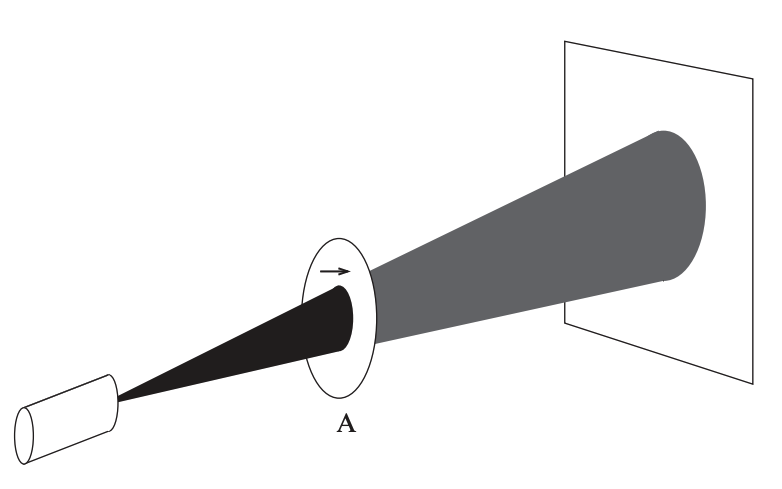
\includegraphics[scale=0.12]{figures/polarization-0}
      \caption{polaroid A with preferred axis $\ket{\rightarrow}$}
      \label{fig:polarization-0}
    \end{subfigure}
    \hfill
    \begin{subfigure}[b]{0.3\textwidth}
      \centering
      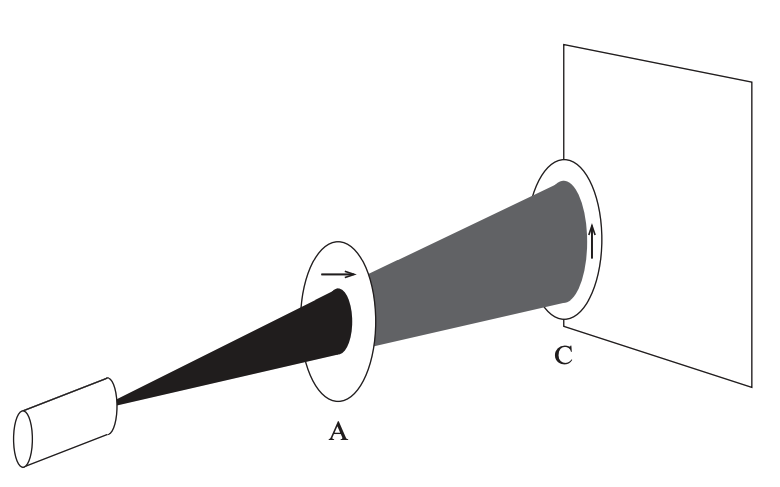
\includegraphics[scale=0.12]{figures/polarization-1}
      \caption{polaroid C with preferred axis $\ket{\uparrow}$}
      \label{fig:polarization-1}
    \end{subfigure}
    \hfill
    \begin{subfigure}[b]{0.3\textwidth}
      \centering
      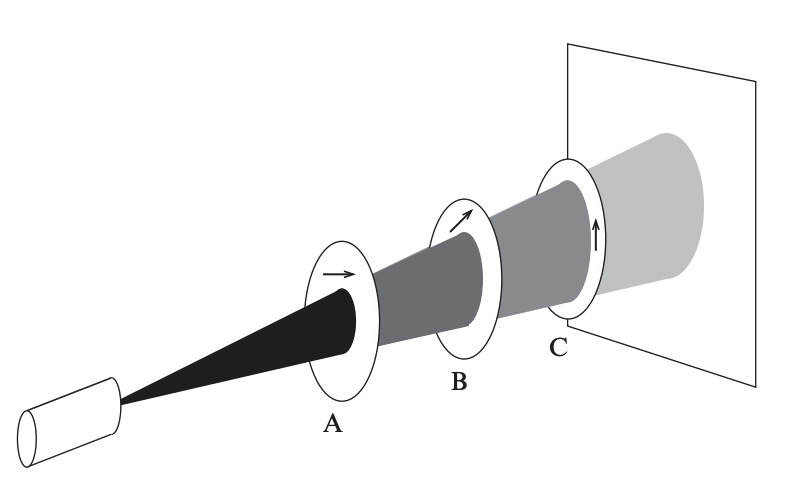
\includegraphics[scale=0.12]{figures/polarization-2}
      \caption{polaroid B with preferred axis $\ket{\nearrow}$}
      \label{fig:polarization-2}
    \end{subfigure}
    \caption{Photon Polarization Experiment\tiny\cite{gentleintroduction}}
    \label{fig:Polarization-3}
  \end{figure}

  \begin{block}{An explanation from quantum mechanics}
    Model a photon (a qubit) as a vector in a 2-dimensional vector space:
    $\ket{v} = a\ket{\uparrow}+ b\ket{\rightarrow}$,
    where $|a|^{2}+|b|^{2}=1$ and \{$\ket{\uparrow}$ and $\ket{\rightarrow}$\} is a basis of the vector space.
    \par
    A polaroid with preferred axis $\ket{\uparrow}$ (like C in figure) can:
    \begin{enumerate}[I]
      \item allow the photon get through with \textbf{possibility} $|a|^2$
      \item absorb the photon with \textbf{possibility} $|b|^2$
      \item polarized the passed photon in direction of $\ket{\uparrow}$
    \end{enumerate}
  \end{block}
\end{frame}

\subsection{Impact of Measurement}
\begin{frame}
  \frametitle{Impact of Measurement}
  \begin{columns}
    \column{0.37\textwidth}
    \begin{figure}
      \centering
      \begin{subfigure}[b]{0.45\textwidth}
        \centering
        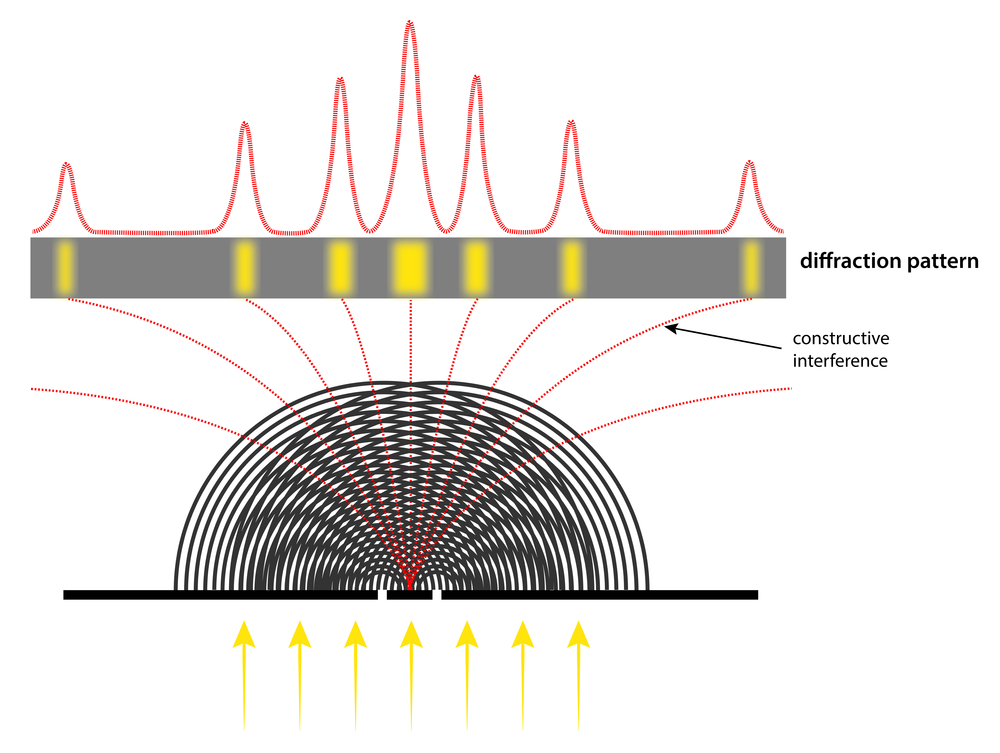
\includegraphics[scale=0.3]{figures/double-slit-0}
        \caption{Double-Slit w/o Detector}
        \label{fig:doube-slit-0}
      \end{subfigure}
      \hfill
      \begin{subfigure}[b]{0.45\textwidth}
        \centering
        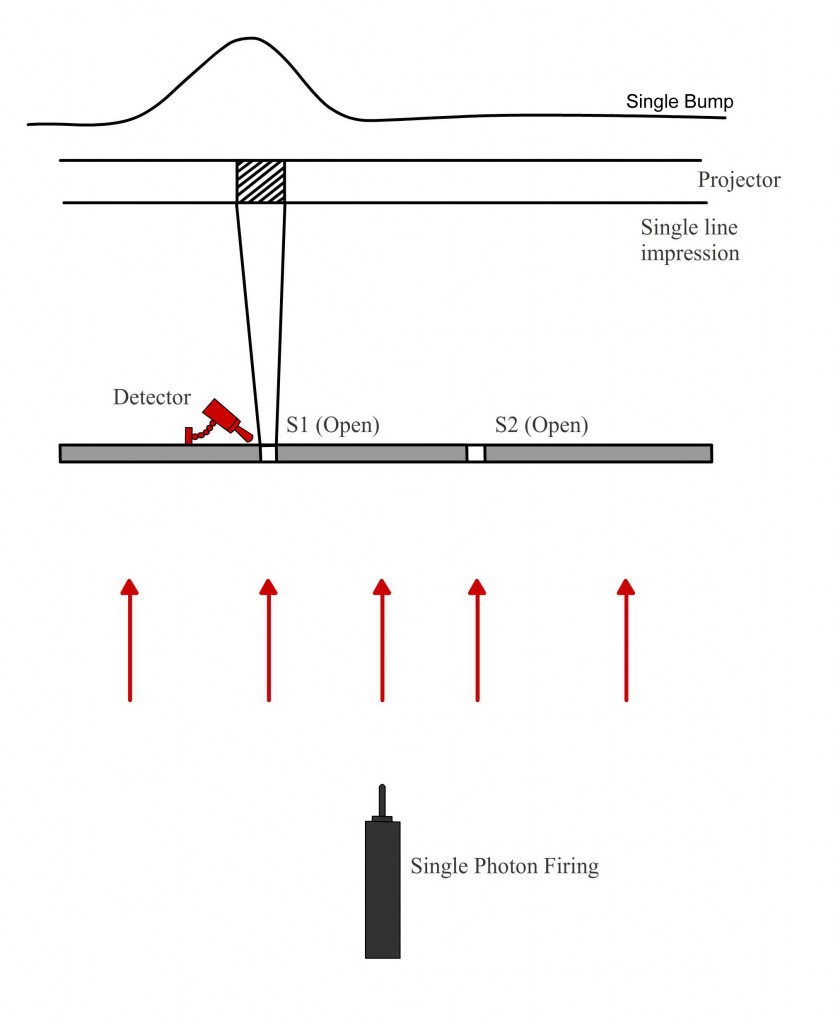
\includegraphics[scale=0.075]{figures/double-slit-1}
        \caption{Double-Slit w/ Detector}
        \label{fig:doube-slit-1}
      \end{subfigure}
      \caption{Double-Slit Experiment\tiny\cite{doubleslit}}
      \label{fig:doube-slit-2}
    \end{figure}
    \begin{figure}
      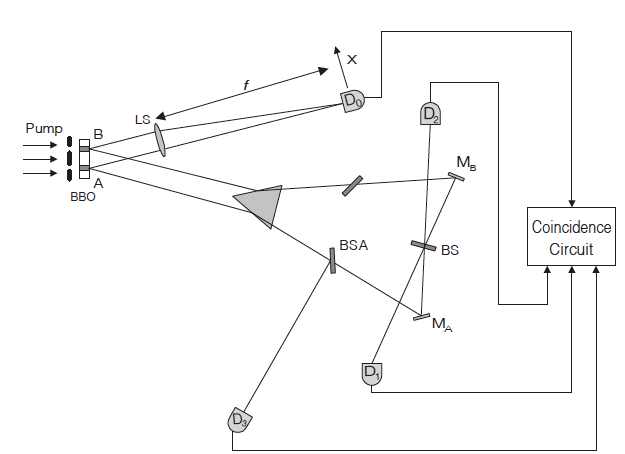
\includegraphics[scale=0.155]{figures/delayed-choice-quantum-eraser}
      \caption{Delayed Choice Quantum Eraser\tiny\cite{delayed}}
    \end{figure}

    \column{0.63\textwidth}
    \begin{block}{Measurement}
      A qubit
        \begin{align*}
        \ket{v} &= a\ket{\uparrow}+ b\ket{\rightarrow} \\
                &= x\ket{\nwarrow}+ y\ket{\nearrow}
        \label{eqn:qubit-bases}
        \end{align*}
      \begin{enumerate}[I]
        \item must be measured in one certain basis, e.g. \{$\ket{\uparrow}$ and $\ket{\rightarrow}$\},
          or \{$\ket{\nwarrow}$ and $\ket{\nearrow}$\};
          the result of measurement is in \textbf{possibility}, which is caused by \textbf{superposition} of the states in a basis.
        \item can be measured once and only once; after being measured, it gives \textbf{deterministic} result, as the quantum system in it has \textbf{decoherented}.
      \end{enumerate}
    \end{block}
  \end{columns}
\end{frame}

\subsection{BB84}
\begin{frame}{BB84: A Quantum Key Distribution Protocol}
  \framesubtitle{The Problem}
  Bob and Alice want to share some secret bits (key). They don't want Eve to know the secret bits.
  \setbeamerfont{block title}{size=\scriptsize}
  \begin{block}{What Bob and Alice can do:}
  {\scriptsize
    \begin{enumerate}[I]
      \item A classical channel to transfer bits.
      \item A quantum channel to transfer qubits.
      \item Encode and measure qubits with Standard basis $\ket{\uparrow}$ and $\ket{\rightarrow}$.
      \item Encode and measure qubits with Hadamard basis $\ket{\nearrow}$ and $\ket{\nwarrow}$.
    \end{enumerate}
  }%
  \end{block}
  \begin{block}{What Eve can do:}
  {\scriptsize
    \begin{enumerate}[I]
      \item Eavesdrop on classical channel.
      \item Eavesdrop a qubit from quantum channel and send another qubit to Bob.
      \item Encode and measure qubits with Standard basis $\ket{\uparrow}$ and $\ket{\rightarrow}$.
      \item Encode and measure qubits with Hadamard basis $\ket{\nearrow}$ and $\ket{\nwarrow}$.
    \end{enumerate}
  }%
  \end{block}
\end{frame}

\begin{frame}{BB84: A Quantum Key Distribution Protocol}
  \setbeamerfont{block title}{size=\scriptsize}
  \begin{block}{How it works}
  {\scriptsize
    \begin{enumerate}[I]
      \item Alice encodes a bit into a qubit with one basis and sends it to Bob through quantum channel;
      \item Eve eavesdrops the qubit and meansures it by \textbf{randomly} picking a basis since she doesn't know the basis Alice used; and then encodes/clones the result into a new qubit with the picked basis and sends it to Bob;
      \item Bob meansures the qubit by randomly picking a basis as well;
      \item through classical channel, Bob tells Alice that the qubit has been received;
      \item through classical channel, Bob and Alice exchange the bases they used;
      \item if they are same basis, the result of measuring the qubit is kept as one basis-matching bit;
      \item else, the result is dropped;
      \item continue steps above until Bob and Alice have enough basis-matching bits;
      \item Bob and Alice agree to select half from those basis-matching bits, and exchange the values of these bits through classical channel;
      \item if there are \textbf{unmatched values}, they are sure about that Eve is eavesdroping;
      \item if there are no unmatched values, it's probably safe to use remaining half of basis-matching bits as final secret bits (key).
    \end{enumerate}
  }%
  \end{block}
\end{frame}

\begin{frame}[fragile]{BB84: How secure the secure bits are?}
  \begin{tikzcd}[row sep=tiny]
    & & & & & & 90 \\
    & & & & 100 \ar[urr, sloped, "matched"] \ar[drr, sloped, "unmatched"] \\
    & & 200 \ar[drr, sloped, "secure\ bits?"] \ar[urr, sloped, "value\ verifying"] & & & & 10 \\
    400 \ar[urr, sloped, "basis\ matched"] \ar[drr, sloped, "basis\ unmatched"'] & & & & 100 \\
    & & 200
  \end{tikzcd}

  \setbeamerfont{block title}{size=\scriptsize}
  \begin{block}{Why there are unmatched values?}
    {\scriptsize
      Because Eve doesn't know the basis Alice used to encode the qubit, she has to pick one basis \textbf{randomly} to encode/clone the qubit again.
      When Eve picked wrong basis, Bob's measurement would get unmatched value in \textbf{possibility}.
      \par
      Can you calculate the possibility exactly?
      \begin{align*}
        \ket{\nearrow} =& \frac{1}{\sqrt{2}}(\ket{\uparrow} + \ket{\rightarrow}) \\
        \ket{\nwarrow} =& \frac{1}{\sqrt{2}}(\ket{\uparrow} - \ket{\rightarrow})
      \end{align*}
    }%
  \end{block}
\end{frame}

\section{Single Qubit System}
\begin{frame}
  Single-Qubit System
\end{frame}

\subsection{Basis}
\begin{frame}{Basis}
  {\tiny
    All possible states of a one-qubit (quantum) system is viewed as a two-dimensional complex vector space. One state can be denated as a vector $\ket{\psi}$ in this space:
  \begin{align*}
    \ket{\psi}&=\alpha\ket{0}+\beta\ket{1} \\
              &=\alpha\begin{bmatrix}1\\0\end{bmatrix}+\beta\begin{bmatrix}0\\1\end{bmatrix}
  \end{align*}
  with \textbf{complex numbers} $\alpha$ and $\beta$, and the normalization constraint $\braket{\psi|\psi}=1$.
  \par
  The $\ket{0}$ and $\ket{1}$, which can be any one pair of \textbf{orthonormal} vectors in this vector space, is a \textbf{basis}.
  }%
\end{frame}

\subsection{Bloch Sphere}
\begin{frame}{State of Single-Qubit System\tiny\cite{blochsphere}}
  \framesubtitle{From 2-Dimensional Complex Vector Space to 3-Dimensional Real Space}
  {\tiny
  A single qubit can be written as:
  \begin{columns}
  \column{0.65\textwidth}
  \begin{align*}
    \ket{\psi} &= \alpha\ket{0}+\beta\ket{1} \\
               &= r_{\alpha}(\cos\phi_{\alpha} + i\,\sin\phi_{\alpha})\ket{0}+\beta\ket{1} \\
               &= r_{\alpha}e^{i\phi_{\alpha}}\ket{0} + r_{\beta}e^{i\phi_{\beta}}\ket{1}
    \\
    e^{-i\phi_{\alpha}}\ket{\psi} &= r_{\alpha}\ket{0} + r_{\beta}e^{i(\phi_{\beta} - \phi_{\alpha})}\ket{1} \\
                                  &= r_{\alpha}\ket{0} + (x+i\,y)\ket{1} \\
                                  &= \ket{\psi'}
  \end{align*}
  $e^{-i\phi_{\alpha}}$ is a \textbf{global phase}, which has no observable consequences.
  \begin{align*}
    \braket{\psi'|\psi'} &= 1 \\
                         &= r_{\alpha}^2 + (x-i\,y)(x+i\,y) \\
                         &= r_{\alpha}^2 + x^2 + y^2
    \\
    \ket{\psi'} &= \cos\theta\ket{0} + \sin\theta(\cos\phi + i\,\sin\phi)\ket{1} \\
                &= \cos\theta\ket{0}+e^{i\phi}\sin\theta\ket{1}
  \end{align*}
  \column{0.35\textwidth}
    \begin{figure}
      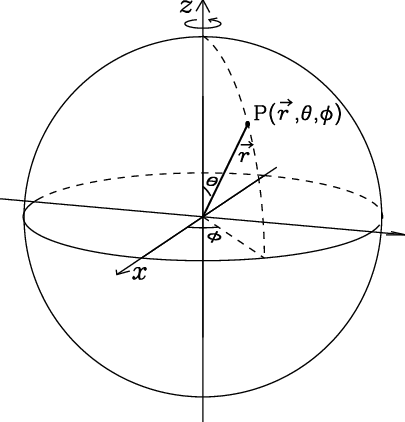
\includegraphics[scale=0.155]{figures/The-spherical-polar-coordinate-system}
      \caption{The spherical polar coordinate system\tiny\cite{sphericalpolarcoordinate}}
    \end{figure}
  \end{columns}
  }%
\end{frame}

\begin{frame}{State of Single-Qubit System\tiny\cite{blochsphere}}
  \framesubtitle{Bloch Sphere}
  {\tiny
  Following is derived already:
  \begin{align*}
    \ket{\psi} &= \cos\theta'\ket{0}+e^{i\phi}\sin\theta'\ket{1} .
  \end{align*}
  When $\theta'=0$, $\ket{\psi}=\ket{0}$; when $\theta'=\frac{\pi}2$, $\ket{\psi}=e^{i\phi}\ket{1}$.
  This suggests there is redundancy in sphere model above.
  Looking at the opposite point of $\ket{\psi}$ on the sphere:
  \begin{align*}
    \ket{\psi'} &= \cos(\pi-\theta')\ket{0}+e^{i(\pi+\phi)}\sin(\pi-\theta')\ket{1} \\
     &= -\cos(\theta')\ket{0}+e^{i\pi}e^{i\phi}\sin\theta'\ket{1} \\
     &= -\cos(\theta')\ket{0}-e^{i\phi}\sin\theta'\ket{1} \\
     &= -\ket{\psi} .
  \end{align*}
  It has only a global phase difference. So a hemisphere is able to represent a qubit. Finally a qubit can be modeled as a \textbf{Bloch Sphere}:
  \begin{align*}
    \ket{\psi} &= \cos(\frac{\theta}2)\ket{0}+e^{i\phi}\sin(\frac{\theta}2)\ket{1}
  \end{align*}
  where $0\leqslant\theta\leqslant\pi$, $0\leqslant\phi\leqslant2\pi$.
  }%
\end{frame}

\begin{frame}{Special States on the Bloch Sphere}
  {\tiny
  $\ket{\psi} = \cos(\frac{\theta}2)\ket{0}+e^{i\phi}\sin(\frac{\theta}2)\ket{1}$, where $0\leqslant\theta\leqslant\pi$, $0\leqslant\phi\leqslant2\pi$.
  \begin{figure}
    \centering
    \begin{subfigure}[b]{0.5\textwidth}
      \centering
      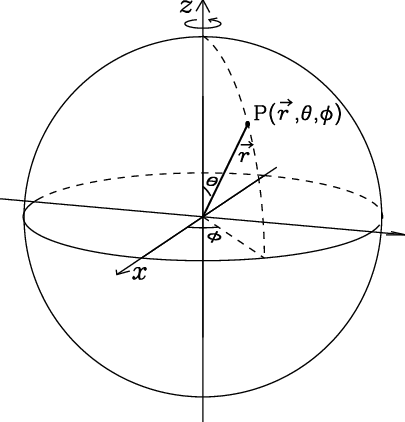
\includegraphics[scale=0.2]{figures/The-spherical-polar-coordinate-system}
      \caption{The spherical polar coordinate system\tiny\cite{sphericalpolarcoordinate}}
    \end{subfigure}
    \hfill
    \begin{subfigure}[b]{0.5\textwidth}
      \centering
      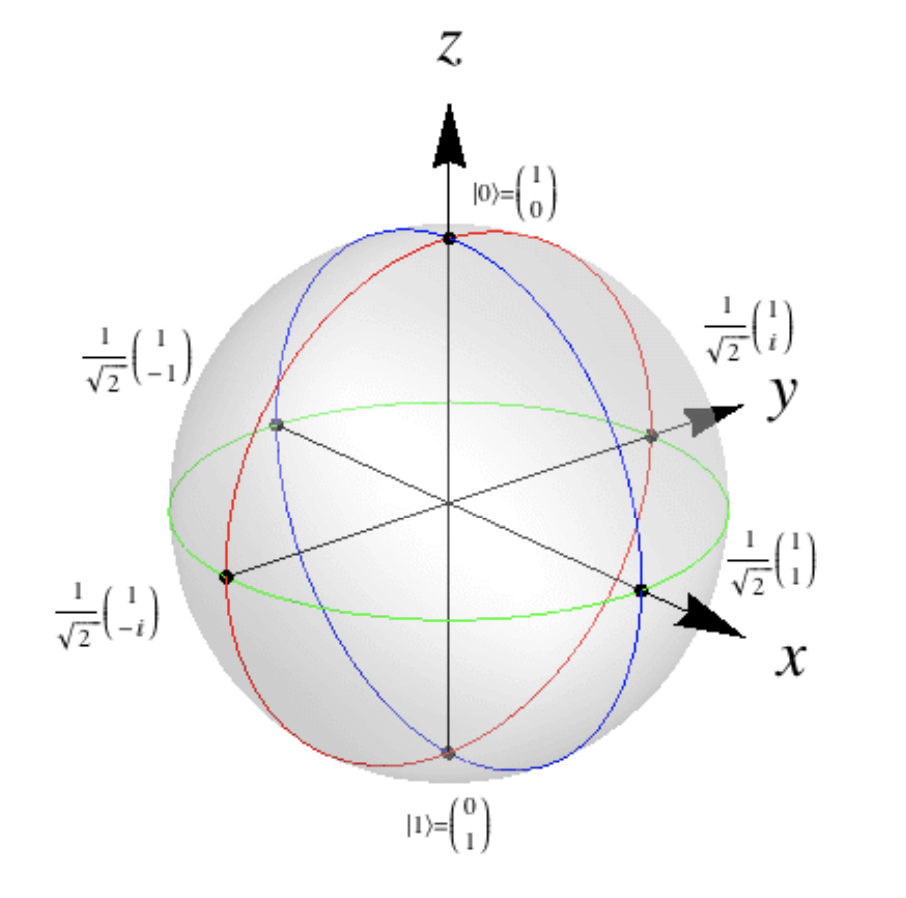
\includegraphics[scale=0.24]{figures/singlequbitstates}
      \caption{The special single qubit states\tiny\cite{singlequbitstates}}
    \end{subfigure}
    \caption{The Block Sphere}
  \end{figure}
  \begin{align*}
  \ket0 &\mapsto \theta = 0                     & \ket1 &\mapsto \theta = \pi \\
  \ket+ &\mapsto \theta = \frac{\pi}2, \phi = 0 & \ket- &\mapsto \theta = \frac{\pi}2, \phi = \pi \\
  \ket{i} &\mapsto \theta = \frac{\pi}2, \phi = \frac{\pi}2 & \ket{-i} &\mapsto \theta = \frac{\pi}2, \phi = \frac{3\pi}2
  \end{align*}
  }%
\end{frame}

\subsection{Rotation on the Bloch Sphere}
\begin{frame}{The Exponential Operator\tiny\cite{rotationsonblochsphere}}
  {\tiny
    Suppose $f(x)$ has a power series $f(x) = \sum_{i=0}^{\infty}c_ix^n$, and define $f(\mathbf{A})$ as:
    \begin{align*}
    f(\mathbf{A}) \equiv c_0\mathbf{I} + c_1\mathbf{A} + c_2\mathbf{A^2} + c_3\mathbf{A^3} + \dots
    \end{align*}
    With Taylor Series:
    \begin{align*}
      \sin{x} &= x - \frac{x^3}{3!} + \frac{x^5}{5!} - \dots \frac{(-1)^kx^{2k+1}}{(2k+1)!}\ \dots \\
      \cos{x} &= 1 - \frac{x^2}{2!} + \frac{x^4}{4!} - \dots \frac{(-1)^kx^{2k}}{(2k)!}\ \dots \\
      e^{ix} &= 1 + \frac{ix}{1!} + \frac{i^2x^2}{2!} + \frac{i^3x^3}{3!}+ \frac{i^4x^4}{4!} + \frac{i^5x^5}{5!} + \dots \\
             &= (1 - \frac{x^2}{2!} + \frac{x^4}{4!} - \dots) + i(x - \frac{x^3}{3!} + \frac{x^5}{5!} - \dots) \\
             &= \cos{x} + i\sin{x}
    \end{align*}
    In case that $\mathbf{A}^2=\mathbf{I}$:
    \begin{align*}
      e^{i\alpha\mathbf{A}} &= \mathbf{I}
                                 + \frac{i\alpha\mathbf{A}}{1!}
                                 + \frac{i^2(\alpha\mathbf{A})^2}{2!}
                                 + \frac{i^3(\alpha\mathbf{A})^3}{3!}
                                 + \frac{i^4(\alpha\mathbf{A})^4}{4!}
                                 + \dots \\
                            &= \cos(\alpha)\mathbf{I} + i\sin(\alpha)\mathbf{A}
    \end{align*}
  }%
\end{frame}

\begin{frame}{The Pauli Matrices and the Rotation Operators\tiny\cite{rotationsonblochsphere}}
  {\tiny
    Given a qubit:
    \begin{align*}
      \ket{\psi} = \cos(\frac{\theta}2)\ket{0}+e^{i\phi}\sin(\frac{\theta}2)\ket{1} &= \begin{bmatrix}\cos{\frac{\theta}2} \\ e^{i\phi}\sin{\frac{\theta}2} \end{bmatrix}
    \end{align*}
    where $0\leqslant\theta\leqslant\pi$, $0\leqslant\phi\leqslant2\pi$, and the exponential operator defined above:
    \begin{align*}
      e^{i\alpha\mathbf{A}} = \cos(\alpha)\mathbf{I} + i\sin(\alpha)\mathbf{A}
    \end{align*}
    Define operators $R_x(\alpha)$, $R_y(\alpha)$ and $R_z(\alpha)$:
    \begin{align*}
      R_x(\alpha) &\equiv \cos\frac{\alpha}2\mathbf{I} - i\sin\frac{\alpha}2
                                                                     \begin{bmatrix}
                                                                       1 & 0 \\
                                                                       0 & 1
                                                                     \end{bmatrix}
                  &= e^{-i\frac{\alpha}2\mathbf{X}}
                  &= \cos\frac{\alpha}2\mathbf{I} - i\sin\frac{\alpha}2 \mathbf{X}
                  &&=\begin{bmatrix}
                    \cos\frac{\alpha}2 & -i\sin\frac{\alpha}2 \\
                    -i\sin\frac{\alpha}2 & \cos\frac{\alpha}2
                    \end{bmatrix} \\
      R_y(\alpha) &\equiv \cos\frac{\alpha}2\mathbf{I} - i\sin\frac{\alpha}2
                                                                     \begin{bmatrix}
                                                                       0 & -i \\
                                                                       i & 0
                                                                     \end{bmatrix}
                  &= e^{-i\frac{\alpha}2\mathbf{Y}}
                  &= \cos\frac{\alpha}2\mathbf{I} - i\sin\frac{\alpha}2 \mathbf{Y}
                  &&=\begin{bmatrix}
                    \cos\frac{\alpha}2 & -\sin\frac{\alpha}2 \\
                    \sin\frac{\alpha}2 & \cos\frac{\alpha}2
                    \end{bmatrix} \\
      R_z(\alpha) &\equiv \cos\frac{\alpha}2\mathbf{I} - i\sin\frac{\alpha}2
                                                                     \begin{bmatrix}
                                                                       1 & 0 \\
                                                                       0 & -1
                                                                     \end{bmatrix}
                  &= e^{-i\frac{\alpha}2\mathbf{Z}}
                  &= \cos\frac{\alpha}2\mathbf{I} - i\sin\frac{\alpha}2 \mathbf{Z}
                  &&=\begin{bmatrix}
                    e^{-i\frac{\alpha}2} & 0 \\
                    0 & e^{i\frac{\alpha}2}
                    \end{bmatrix} \\
    \end{align*}
    The $\mathbf{X}$, $\mathbf{Y}$, and $\mathbf{Z}$ are Pauli Matrices.
  }%
\end{frame}

\begin{frame}{An Example of Rotation\tiny\cite{rotationsonblochsphere}}
  {\tiny
    Rotate $\ket\psi$ about z-axis by angle of $\alpha$ on the Bloch Sphere:
  \begin{align*}
    R_z(\alpha)\ket{\psi} &= \begin{bmatrix}
                                e^{-i\frac{\alpha}2} & 0 \\
                                0                    & e^{i\frac{\alpha}2}
                              \end{bmatrix}
                              \begin{bmatrix}
                                \cos{\frac{\theta}2} \\
                                e^{i\phi}\sin{\frac{\theta}2}
                              \end{bmatrix} \\
                          &= \begin{bmatrix}
                               e^{-i\frac{\alpha}2}\cos{\frac{\theta}2} \\
                               e^{i\frac{\alpha}2}\sin{\frac{\theta}2}
                             \end{bmatrix} \\
     e^{i\frac{\alpha}2}R_z(\alpha)\ket{\psi}
                          &= \begin{bmatrix}
                               \cos{\frac{\theta}2} \\
                               e^{i\alpha}e^{i\phi}\sin{\frac{\theta}2}
                             \end{bmatrix} \\
    \\
    R_x(\alpha)\ket{\psi} &= \begin{bmatrix}
                              \cos\frac{\alpha}2 & -i\sin\frac{\alpha}2 \\
                              -i\sin\frac{\alpha}2 & \cos\frac{\alpha}2
                             \end{bmatrix}
                             \begin{bmatrix}
                               \cos{\frac{\theta}2} \\
                               e^{i\phi}\sin{\frac{\theta}2}
                             \end{bmatrix} \\
                             &= \begin{bmatrix}
                               \cos\frac{\alpha}2 \cos\frac{\theta}2 - i e^{i\phi} \sin\frac{\alpha}2 \sin\frac{\theta}2 \\
                               -i \sin\frac{\alpha}2 \cos\frac{\theta}2 + e^{i\phi} \cos\frac{\alpha}2 \sin\frac{\theta}2
                                \end{bmatrix} \\
                             &= \dots
  \end{align*}
  }%
\end{frame}

\begin{frame}{The Density Operator\tiny\cite{rotationsonblochsphere}}
  {\tiny
  Another representation of a qubit state $\ket{\psi}$:
    \begin{align*}
      \rho &= \ket{\psi} \otimes \bra{\psi} = \ket{\psi} \otimes \ket{\psi}^{\dagger} \\
           &= \begin{bmatrix}
                \cos{\frac{\theta}2} \\
                e^{i\phi}\sin{\frac{\theta}2}
              \end{bmatrix}
              \otimes
              \begin{bmatrix}
                \cos{\frac{\theta}2} & e^{-i\phi}\sin{\frac{\theta}2}
              \end{bmatrix} \\
           &= \begin{bmatrix}
                \cos^2{\frac{\theta}2}                            & e^{-i\phi}\cos{\frac{\theta}2}\sin{\frac{\theta}2} \\
                e^{i\phi}\cos{\frac{\theta}2}\sin{\frac{\theta}2} & \sin^2{\frac{\theta}2}
              \end{bmatrix} \\
           &= \begin{bmatrix}
                \frac{1+\cos{\theta}}2                       & (\cos{\phi}-i\sin{\phi})\frac{\sin\theta}2 \\
                (\cos{\phi}+i\sin{\phi})\frac{\sin\theta}2   & \frac{1-\cos{\theta}}2
              \end{bmatrix} \\
           &= \frac{1}2
              \begin{pmatrix}
                \begin{bmatrix}
                  1 & 0 \\
                  0 & 1
                \end{bmatrix}
                +
                \cos\phi\sin\theta
                \begin{bmatrix}
                  0 & 1 \\
                  1 & 0
                \end{bmatrix}
                +
                \sin\phi\sin\theta
                \begin{bmatrix}
                  0 & -i \\
                  i & 0
                \end{bmatrix}
                +
                \cos\theta
                \begin{bmatrix}
                  1 & 0 \\
                  0 & -1
                \end{bmatrix}
              \end{pmatrix} \\
            &= \frac{1}2(\mathbf{I} + \mathbf{X}\cos\phi\sin\theta + \mathbf{Y}\sin\phi\sin\theta + \mathbf{Z}\cos\theta) \\
            &= \frac{1}2(\mathbf{I} + (\mathbf{X}, \mathbf{Y}, \mathbf{Z}) \cdot (r_x, r_y, r_z)) \\
            &= \frac{1}2 ( \mathbf{I} + \overrightarrow{\sigma} \cdot \overrightarrow{\mathbf{r}}_{\rho} )
    \end{align*}
  }%
\end{frame}

\begin{frame}{Rotation with the Density Operator - I\tiny{\cite{rotationsonblochsphere}}}
  {\tiny
    For rotation $R_z(\alpha)$:
    \begin{columns}
    \column{0.7\textwidth}
    \begin{align*}
      \rho' &= R_z(\alpha)\ket{\psi} \otimes (R_z(\alpha)\ket{\psi})^{\dagger} \\
            &= R_z(\alpha)(\ket{\psi} \otimes \bra{\psi})R_z(\alpha)^{\dagger} \\
            &= R_z(\alpha) \rho R_z(\alpha)^{\dagger} \\
            &= \frac{1}2(\mathbf{I}  + r_x R_z(\alpha) \mathbf{X} R_z(\alpha)^{\dagger}
                                     + r_y R_z(\alpha) \mathbf{Y} R_z(\alpha)^{\dagger}
                                     + r_z R_z(\alpha) \mathbf{Z} R_z(\alpha)^{\dagger} \\
      \\
      R_z(\alpha) \mathbf{X} R_z(\alpha)^{\dagger}
            &=    \begin{pmatrix} \cos\frac{\alpha}2\mathbf{I} - i\sin\frac{\alpha}2 \mathbf{Z} \end{pmatrix}
                  \mathbf{X}
                  \begin{pmatrix} \cos\frac{\alpha}2\mathbf{I} + i\sin\frac{\alpha}2 \mathbf{Z} \end{pmatrix} \\
            &=    \cos^2\frac{\alpha}2 \mathbf{X}
                + i\sin\frac{\alpha}2 \cos\frac{\alpha}2 \mathbf{X}\mathbf{Z}
                - i\sin\frac{\alpha}2 \cos\frac{\alpha}2 \mathbf{Z}\mathbf{X}
                + \sin^2\frac{\alpha}2 \mathbf{Z}\mathbf{X}\mathbf{Z} \\
            &=    \begin{pmatrix} \cos^2\frac{\alpha}2 -  \sin^2\frac{\alpha}2 \end{pmatrix} \mathbf{X}
                + 2 \sin\frac{\alpha}2 \cos\frac{\alpha}2 \mathbf{Y} \\
            &= \cos\alpha \mathbf{X} + \sin\alpha \mathbf{Y} \\
      R_z(\alpha) \mathbf{Y} R_z(\alpha)^{\dagger}
            &=    \cos\alpha \mathbf{Y} - \sin\alpha \mathbf{X} \\
      R_z(\alpha) \mathbf{Z} R_z(\alpha)^{\dagger}
            &=    \begin{pmatrix} \cos\frac{\alpha}2\mathbf{I} - i\sin\frac{\alpha}2 \mathbf{Z} \end{pmatrix}
                  \mathbf{Z}
                  \begin{pmatrix} \cos\frac{\alpha}2\mathbf{I} + i\sin\frac{\alpha}2 \mathbf{Z} \end{pmatrix} \\
            &=    \cos^2\frac{\alpha}2 \mathbf{Z}
                + i\sin\frac{\alpha}2 \cos\frac{\alpha}2 \mathbf{Z}\mathbf{Z}
                - i\sin\frac{\alpha}2 \cos\frac{\alpha}2 \mathbf{Z}\mathbf{Z}
                + \sin^2\frac{\alpha}2 \mathbf{Z}\mathbf{Z}\mathbf{Z} \\
            &=    \mathbf{Z} \\
      \\
      \rho' &= \frac{1}2 ( \mathbf{I} + \overrightarrow{\sigma} \cdot \overrightarrow{\mathbf{r}}_{\rho'} )
            , where \overrightarrow{\mathbf{r}}_{\rho'} =
              \begin{bmatrix}
                \cos\alpha & -\sin\alpha & 0 \\
                \sin\alpha & \cos\alpha  & 0 \\
                0          & 0           & 1
              \end{bmatrix}
              \overrightarrow{\mathbf{r}}_{\rho}
    \end{align*}
    \column{0.3\textwidth}
    \setbeamerfont{block title}{size=\tiny}
    \begin{block}{The Algebra of the Pauli Matrices}
      $\mathbf{X}^2 = \mathbf{Y}^2 = \mathbf{Z}^2 = -i\mathbf{XYZ} = \mathbf{I}$ \\
      $\mathbf{XY} = -\mathbf{YX} = i\mathbf{Z}$ \\
      $\mathbf{YZ} = -\mathbf{ZY} = i\mathbf{X}$ \\
      $\mathbf{ZX} = -\mathbf{XZ} = i\mathbf{Y}$
    \end{block}
    \end{columns}
  }%
\end{frame}

\begin{frame}{Rotation with the Density Operator - II}
  {\tiny
    For rotation $R_x(\alpha)$:
    \begin{align*}
      \rho' &= R_x(\alpha) \rho R_x(\alpha)^{\dagger} \\
            &= \frac{1}2(\mathbf{I}  + r_x R_x(\alpha) \mathbf{X} R_x(\alpha)^{\dagger}
                                     + r_y R_x(\alpha) \mathbf{Y} R_x(\alpha)^{\dagger}
                                     + r_z R_x(\alpha) \mathbf{Z} R_x(\alpha)^{\dagger} \\
      \\
      R_x(\alpha) \mathbf{X} R_x(\alpha)^{\dagger}
            &=  \begin{pmatrix} \cos\frac{\alpha}2\mathbf{I} - i\sin\frac{\alpha}2 \mathbf{X} \end{pmatrix}
                \mathbf{X}
                \begin{pmatrix} \cos\frac{\alpha}2\mathbf{I} + i\sin\frac{\alpha}2 \mathbf{X} \end{pmatrix} \\
            &=    \cos^2\frac{\alpha}2 \mathbf{X}
                + i\sin\frac{\alpha}2 \cos\frac{\alpha}2 \mathbf{X}\mathbf{X}
                - i\sin\frac{\alpha}2 \cos\frac{\alpha}2 \mathbf{X}\mathbf{X}
                + \sin^2\frac{\alpha}2 \mathbf{X}\mathbf{X}\mathbf{X} \\
            &= X \\
      R_x(\alpha) \mathbf{Y} R_x(\alpha)^{\dagger}
            &=  \begin{pmatrix} \cos\frac{\alpha}2\mathbf{I} - i\sin\frac{\alpha}2 \mathbf{X} \end{pmatrix}
                \mathbf{Y}
                \begin{pmatrix} \cos\frac{\alpha}2\mathbf{I} + i\sin\frac{\alpha}2 \mathbf{X} \end{pmatrix} \\
            &=    \cos^2\frac{\alpha}2 \mathbf{Y}
                + i\sin\frac{\alpha}2 \cos\frac{\alpha}2 \mathbf{Y}\mathbf{X}
                - i\sin\frac{\alpha}2 \cos\frac{\alpha}2 \mathbf{X}\mathbf{Y}
                + \sin^2\frac{\alpha}2 \mathbf{X}\mathbf{Y}\mathbf{X} \\
            &=    \cos^2\frac{\alpha}2 \mathbf{Y}
                + \sin\frac{\alpha}2 \cos\frac{\alpha}2 \mathbf{Z}
                + \sin\frac{\alpha}2 \cos\frac{\alpha}2 \mathbf{Z}
                - \sin^2\frac{\alpha}2 \mathbf{Y} \\
            &=    \cos\alpha \mathbf{Y} + \sin\alpha \mathbf{Z} \\
      R_z(\alpha) \mathbf{Z} R_z(\alpha)^{\dagger}
            &=    \cos\alpha \mathbf{Z} - \sin\alpha \mathbf{Y} \\
      \\
      \rho' &= \frac{1}2 ( \mathbf{I} + \overrightarrow{\sigma} \cdot \overrightarrow{\mathbf{r}}_{\rho'} )
            , where \overrightarrow{\mathbf{r}}_{\rho'} =
              \begin{bmatrix}
                1 & 0          & 0 \\
                0 & \cos\alpha & -\sin\alpha \\
                0 & \sin\alpha & \cos\alpha \\
              \end{bmatrix}
              \overrightarrow{\mathbf{r}}_{\rho}
    \end{align*}
  }%
\end{frame}

\begin{frame}{Rotation with the Density Operator - III}
  {\tiny
    For rotation $R_y(\alpha)$:
    \begin{align*}
      \rho' &= R_y(\alpha) \rho R_y(\alpha)^{\dagger} \\
            &= \frac{1}2(\mathbf{I}  + r_x R_y(\alpha) \mathbf{X} R_y(\alpha)^{\dagger}
                                     + r_y R_y(\alpha) \mathbf{Y} R_y(\alpha)^{\dagger}
                                     + r_z R_y(\alpha) \mathbf{Z} R_y(\alpha)^{\dagger} \\
      \\
      R_y(\alpha) \mathbf{X} R_y(\alpha)^{\dagger}
            &=    \begin{pmatrix} \cos\frac{\alpha}2\mathbf{I} - i\sin\frac{\alpha}2 \mathbf{Y} \end{pmatrix}
                  \mathbf{X}
                  \begin{pmatrix} \cos\frac{\alpha}2\mathbf{I} + i\sin\frac{\alpha}2 \mathbf{Y} \end{pmatrix} \\
            &=    \cos^2\frac{\alpha}2 \mathbf{X}
                + i\sin\frac{\alpha}2 \cos\frac{\alpha}2 \mathbf{X}\mathbf{Y}
                - i\sin\frac{\alpha}2 \cos\frac{\alpha}2 \mathbf{Y}\mathbf{X}
                + \sin^2\frac{\alpha}2 \mathbf{Y}\mathbf{X}\mathbf{Y} \\
            &=    \cos^2\frac{\alpha}2 \mathbf{X}
                - \sin\frac{\alpha}2 \cos\frac{\alpha}2 \mathbf{Z}
                - \sin\frac{\alpha}2 \cos\frac{\alpha}2 \mathbf{Z}
                - \sin^2\frac{\alpha}2 \mathbf{X} \\
            &=    \cos\alpha \mathbf{X} - \sin\alpha \mathbf{Z} \\
      R_y(\alpha) \mathbf{Y} R_y(\alpha)^{\dagger}
            &= Y \\
      R_y(\alpha) \mathbf{Z} R_y(\alpha)^{\dagger}
            &=    \begin{pmatrix} \cos\frac{\alpha}2\mathbf{I} - i\sin\frac{\alpha}2 \mathbf{Y} \end{pmatrix}
                  \mathbf{Z}
                  \begin{pmatrix} \cos\frac{\alpha}2\mathbf{I} + i\sin\frac{\alpha}2 \mathbf{Y} \end{pmatrix} \\
            &=    \cos^2\frac{\alpha}2 \mathbf{Z}
                + i\sin\frac{\alpha}2 \cos\frac{\alpha}2 \mathbf{Z}\mathbf{Y}
                - i\sin\frac{\alpha}2 \cos\frac{\alpha}2 \mathbf{Y}\mathbf{Z}
                + \sin^2\frac{\alpha}2 \mathbf{Y}\mathbf{Z}\mathbf{Y} \\
            &=    \cos^2\frac{\alpha}2 \mathbf{Z}
                + \sin\frac{\alpha}2 \cos\frac{\alpha}2 \mathbf{X}
                + \sin\frac{\alpha}2 \cos\frac{\alpha}2 \mathbf{X}
                - \sin^2\frac{\alpha}2 \mathbf{Z} \\
            &= \cos\alpha \mathbf{Z} + \sin\alpha \mathbf{X} \\
      \\
      \rho' &= \frac{1}2 ( \mathbf{I} + \overrightarrow{\sigma} \cdot \overrightarrow{\mathbf{r}}_{\rho'} )
            , where \overrightarrow{\mathbf{r}}_{\rho'} =
              \begin{bmatrix}
                \cos\alpha  & 0 & \sin\alpha \\
                0           & 1 & 0 \\
                -\sin\alpha & 0 & \cos\alpha \\
              \end{bmatrix}
              \overrightarrow{\mathbf{r}}_{\rho}
    \end{align*}
  }%
\end{frame}

\section{Multiple-Qubit System}
\begin{frame}
  Multiple-Qubit System
\end{frame}

\subsection{Tensor Product}
\begin{frame}{Tensor Product}
  {\tiny
    If A is a $m \times n$ matrix and B a $m' \times n'$ matrix, then their tensor product $\otimes$ is a $mm' \times nn'$ matrix
    \begin{align*}
      A \otimes B = \begin{bmatrix}
                      A_{11}B & \dots & A_{1n}B \\
                      A_{21}B & \dots & A_{2n}B \\
                              & \ddots &        \\
                      A_{m1}B & \dots & A_{mn}B \\
                    \end{bmatrix}
    \end{align*}
    Examples:
    \begin{align*}
      \begin{bmatrix} 1 \\ 0 \end{bmatrix} \otimes \begin{bmatrix} 1 \\ 0 \end{bmatrix} &=
          \begin{bmatrix}
            1 \begin{bmatrix} 1 \\ 0 \end{bmatrix} \\
            \\
            0 \begin{bmatrix} 1 \\ 0 \end{bmatrix}
          \end{bmatrix}
          = \begin{bmatrix} 1 \\ 0 \\ 0 \\ 0 \end{bmatrix} \\
      \begin{bmatrix} 1 \\ 0 \end{bmatrix} \begin{bmatrix} 1 & 0 \end{bmatrix} &= \begin{bmatrix}
                                                                                    1 & 0 \\
                                                                                    0 & 0
                                                                                  \end{bmatrix} \\
      \begin{bmatrix} 1 \\ 0 \end{bmatrix} \otimes \begin{bmatrix} 0 \\ 1 \\ 0 \\ 0 \end{bmatrix} &=
          \begin{bmatrix}
            1 \begin{bmatrix} 0 \\ 1 \\ 0 \\ 0 \end{bmatrix} \\
            \\
            0 \begin{bmatrix} 0 \\ 1 \\ 0 \\ 0 \end{bmatrix}
          \end{bmatrix}
          = \begin{bmatrix} 0 \\ 1 \\ 0 \\ 0 \\ 0 \\ 0 \\ 0 \\ 0 \end{bmatrix} \\
      \begin{bmatrix} 1 \\ 0 \end{bmatrix} \begin{bmatrix} 0 & 1 & 0 & 0 \end{bmatrix} &= \begin{bmatrix}
                                                                                            0 & 1 & 0 & 0\\
                                                                                            0 & 0 & 0 & 0
                                                                                          \end{bmatrix}
    \end{align*}
  }%
\end{frame}

\subsection{State Space of Qubit System}
\begin{frame}{State Space of 2-Qubit System}
  {\tiny
  All possible states of a single-qubit system is viewed as a two-dimensional complex vector space.
  All possible states of a 2-qubit system is viewed as the tensor product ($\otimes$) of two such vector spaces.
  This tensor product is a vecor space as well. Its dimension is $2^2$.\\
  Let $\mathbf{V}$ and $\mathbf{W}$ be two-dimensional complex vector spaces with
  bases $A=\{\ket{\alpha_1}, \ket{\alpha_2}\}$ and $B=\{\ket{\beta_1}, \ket{\beta_2}\}$ respectively. \\
  One basis of $\mathbf{V} \otimes \mathbf{W}$ is:
  \begin{align*}
    \{\ket\alpha_1 \otimes \ket\beta_1,
       \ket\alpha_1 \otimes \ket\beta_2,
       \ket\alpha_2 \otimes \ket\beta_1,
       \ket\alpha_2 \otimes \ket\beta_2 \}
  \end{align*}
  With standard basis on both vector spaces, one basis of the tensor product is defined as:
  \begin{align*}
    \{\ket0 \otimes \ket0, \ket0 \otimes \ket1, \ket1 \otimes \ket0, \ket1 \otimes \ket1 \}
    &= \{\ket{00}, \ket{01}, \ket{10}, \ket{11} \} \\
    &= \{
      \begin{bmatrix} 1 \\ 0 \\ 0 \\ 0 \end{bmatrix},
      \begin{bmatrix} 0 \\ 1 \\ 0 \\ 0 \end{bmatrix},
      \begin{bmatrix} 0 \\ 0 \\ 1 \\ 0 \end{bmatrix},
      \begin{bmatrix} 0 \\ 0 \\ 0 \\ 1 \end{bmatrix}
    \}
  \end{align*}
  Examples (Tensor Product: Vector $\ket{v} \otimes \ket{w}$ vs Vector Space $\mathbf{V} \otimes \mathbf{W}$): \\
  Let state $\ket{v}=a_1\ket0 + a_2\ket1$ and state $\ket{w}=b_1\ket0 + b_2\ket1$, the tensor product of these two states is:
  \begin{align*}
  a_1b_1\ket{00} + a_1b_2\ket{01} + a_2b_1\ket{10} + a_2b_2\ket{11}
  \end{align*}
  Can you find $a_1$, $a_2$, $b_1$, and $b_2$ which satisfy following?
  \begin{align*}
  (a_1\ket0 + a_2\ket1) \otimes (b_1\ket0 + b_2\ket1) = \frac{1}{\sqrt2}(\ket{00} + \ket{11})
  \end{align*}
  It turns out that most \textbf{states} of a 2-qubit quantum system cannot be described in terms of the \textbf{states} of two separate single-qubit systems.
  These states stand for \textbf{entanglement} of the 2-qubit quantum system.
  }%
\end{frame}

\begin{frame}{State Space of N-Qubit System}
  {\tiny
  The standard basis for an n-qubit system is written as
  \begin{align*}
    \{\ket{0\dots00}, \ket{0\dots01}, \ket{0\dots10}, \dots, \ket{1\dots11}\}
  \end{align*}
  or
  \begin{align*}
    \{\ket{0}, \ket{1}, \ket{2}, \dots, \ket{2^{n-1}}\}
  \end{align*}
  Example:
  \begin{align*}
    \frac{1}{2} (\ket{1} + \ket{2} + \ket{4} + \ket{7}) = \frac{1}{2} (\ket{001} + \ket{010} + \ket{100} + \ket{111})
  \end{align*}
  We use the standard basis predominantly, but we use other bases from time to time. E.g. Bell basis:
  \begin{align*}
    \ket{\Phi^+} &= 1/\sqrt2(\ket{00} + \ket{11}) \\
    \ket{\Phi^-} &= 1/\sqrt2(\ket{00} - \ket{11}) \\
    \ket{\Psi^+} &= 1/\sqrt2(\ket{01} + \ket{10}) \\
    \ket{\Psi^-} &= 1/\sqrt2(\ket{01} - \ket{10})
  \end{align*}
  }%
\end{frame}

\begin{frame}{Develop Our Understanding on Superposition}
  {\tiny
  Superposition can not be described as in multiple states “at the same time”. It is not probabilistic mixture. It is only caused by what we human beings can observe/measure.
  Consider
  \begin{align*}
    \frac{1}{\sqrt{2}} (\ket{00} + \ket{11}) \\
    \frac{1}{\sqrt{2}} (\ket{00} + \textbf{i}\ket{11})
  \end{align*}.
  They behave differently under a variety of circumstances. And 
  \begin{align*}
    \frac{1}{\sqrt{2}} (\ket{00} + \ket{11}) \\
    \frac{1}{\sqrt{2}} (\ket{++} + \ket{--})
  \end{align*}
  represent the same state of a quantum system. Thus they behave precisely same at all circumstances.
  }%
\end{frame}

\subsection{Entanglement}
\begin{frame}{Entanglement}
  {\tiny
    Example: A 4-qubit system
    \begin{align*}
      \ket{\Psi} &= \frac{1}{2} (\ket{00} + \ket{11} + \ket{22} + \ket{33}) \\
                 &= \frac{1}{2} (\ket{0}_1\ket{0}_2\ket{0}_3\ket{0}_4 + \ket{0}_1\ket{1}_2\ket{0}_3\ket{1}_4 + \ket{1}_1\ket{0}_2\ket{1}_3\ket{0}_4 + \ket{1}_1\ket{1}_2\ket{1}_3\ket{1}_4 \\
                   &  \text{(Can't be written as decomposition of 4 1-qubit systems)} \\
                   &  \text{(Can be written as decomposition of 2 2-qubit systems)} \\
                 &= \frac{1}{\sqrt{2}} (\ket{0}_1\ket{0}_3  + \ket{1}_1\ket{1}_3) \otimes  \frac{1}{\sqrt{2}} (\ket{0}_2\ket{0}_4  + \ket{1}_2\ket{1}_4) \\
                 &= \frac{1}{2} ( \begin{bmatrix} 1 \\ 0 \\ 0 \\ 0 \end{bmatrix}_{13} \otimes  \begin{bmatrix} 1 \\ 0 \\ 0 \\ 0 \end{bmatrix}_{24} +
                                  \begin{bmatrix} 1 \\ 0 \\ 0 \\ 0 \end{bmatrix}_{13} \otimes  \begin{bmatrix} 0 \\ 0 \\ 0 \\ 1 \end{bmatrix}_{24} +
                                  \begin{bmatrix} 0 \\ 0 \\ 0 \\ 1 \end{bmatrix}_{13} \otimes  \begin{bmatrix} 1 \\ 0 \\ 0 \\ 0 \end{bmatrix}_{24} +
                                  \begin{bmatrix} 0 \\ 0 \\ 0 \\ 1 \end{bmatrix}_{13} \otimes  \begin{bmatrix} 0 \\ 0 \\ 0 \\ 1 \end{bmatrix}_{24} )
    \end{align*}

    “Strictly speaking, entanglement is always with respect to a specified tensor product decomposition of the state \textbf{space}.
    More formally, given a state $\ket\psi$ of some quantum system with associated vector space V and a tensor decomposition of V, $V = V_1 \otimes \dots \otimes V_n$,
    the state $\ket\psi$ is separable, or unentangled, with respect to that decomposition if it can be written as \\
    $\ket\psi = \ket{v_1} \otimes \dots \otimes \ket{v_n} $, where $\ket{v_i}$ is contained in $V_i$. Otherwise, $\ket\psi$ is entangled with respect to this decomposition.”
    \par
    “\dots; states entangled with respect to the single-qubit decomposition may be unentangled with respect to other decompositions into subsystems.”
    \par
    “It is important to recognize that the notion of entanglement is \textbf{NOT} basis dependent, even though it depends on the tensor decomposition under consideration;”
  }%
\end{frame}

\begin{frame}{SVD: Singular Value Decomposition: Preparation}
  \framesubtitle{Review knowledge Learned in School}
  {\tiny
  \begin{block}{}
    If $\textbf{v}_1,\dots,\textbf{v}_r$ are eigenvectors that correspond to distinct eigenvalues $\lambda_1,\dots,\lambda_r$ of an $n{\times}n$ matrix A, then the set ${\textbf{v}_1,\dots,\textbf{v}_r}$ is linearly independent.
  \end{block}
  \begin{block}{}
    An $n{\times}n$ matrix A is diagonalizable ($A=PDP^{-1}$) if and only if A has n linearly independent eigenvectors.
  \end{block}
  \begin{block}{}
    If A is symmetric ($A^T=A$), then any two eigenvectors from different eigenspaces are orthogonal.
    \begin{align*}
      \lambda_1 \textbf{v}_1 \cdot \textbf{v}_2 &= (\lambda_1 \textbf{v}_1)^T \textbf{v}_2 = (A \textbf{v}_1)^T \textbf{v}_2 = \textbf{v}_1^T A^T \textbf{v}_2 \\
                                                &= \textbf{v}_1^T A \textbf{v}_2 = \textbf{v}_1^T (\lambda_2 \textbf{v}_2) = \lambda_2 \textbf{v}_1^T \textbf{v}_2 \\
                                                &= \lambda_2 \textbf{v}_1 \cdot \textbf{v}_2
    \end{align*}
  \end{block}
  \begin{block}{}
    An $n{\times}n$ matrix A is orthogonally diagonalizable if and only if A is a symmetric matrix.
    \begin{enumerate}[I]
      \item $A = PDP^T = PDP^{-1}$
      \item $A$ has $n$ real eigenvalues, counting multiplicities.
      \item The eigenspaces are mutually orthogonal, in the sense that eigenvectors corresponding to different eigenvalues are orthogonal.
    \end{enumerate}
  \end{block}
  }%
\end{frame}

\begin{frame}{SVD: Singular Value Decomposition}
  \framesubtitle{Review knowledge Learned in School}
  {\tiny
    Let A be an $m{\times}n$ matrix. Then $A^{T}A$ is $n{\times}n$ symmetric matrix. Let $\{\textbf{v}_1,\dots,\textbf{v}_n\}$ be an orthonormal basis for $\mathbb{R}^n$ consisting of eigenvectors of $A^{T}A$, and let $\lambda_1,\dots,\lambda_n$ be the associated eigenvalues of $A^{T}A$.
    Then, for $1 \leq i \leq n$,
    \begin{align*}
      \Vert A \textbf{v}_i \Vert^2 &= (A \textbf{v}_i)^T A \textbf{v}_i = \textbf{v}_i^T (A^T A \textbf{v}_i) = \textbf{v}_i^T (\lambda_i \textbf{v}_i) \\
                                   &= \lambda_i
    \end{align*}
    These eigenvalues of $A^TA$ can be arranged to satisfy $\lambda_1 \geq \dots \geq \lambda_n \geq 0$.
    Suppose there are r nonzero eigenvalues ${\lambda_1,\dots,\lambda_r}$, and let $\sigma_i = \sqrt{\lambda_i}$, then
    \begin{align*}
      \textbf{u}_i &= \frac{1}{\Vert A \textbf{v}_i \Vert} A \textbf{v}_i = \frac{1}{\sigma_i} A \textbf{v}_i
    \end{align*}
    and $A \textbf{v}_i = \sigma_i \textbf{u}_i \quad ( 1 \leq i \leq r)$.
    Now extend $\{\textbf{u}_1,\dots,\textbf{u}_r\}$ to an orthonormal basis $\{\textbf{u}_1,\dots,\textbf{u}_r,\dots,\textbf{u}_m\}$ of $\mathbb{R}^m$, and then
    \begin{align*}
      U\Sigma &=
      \begin{bmatrix} \textbf{u}_1 & \textbf{u}_1 & \dots & \textbf{u}_m \end{bmatrix}
      \begin{bmatrix}
        \sigma_1   &        & 0          & 0      \\
                   & \ddots &            & \vdots \\
        0          &        & \sigma_r   & 0      \\
        0          & \cdots & 0          & 0
      \end{bmatrix} \\
      &= \begin{bmatrix} \sigma_1 \textbf{u}_1 & \dots & \sigma_r \textbf{u}_r & \textbf{0} & \dots & \textbf{0} \end{bmatrix} \\
      &= \begin{bmatrix} A \textbf{v}_1        & \dots & A \textbf{v}_r        & \textbf{0} & \dots & \textbf{0} \end{bmatrix} = AV \\
      A &= U \Sigma V^T
         =  \begin{bmatrix} \textbf{u}_1 & \textbf{u}_1 & \dots & \textbf{u}_m \end{bmatrix} 
            \begin{bmatrix}
              \sigma_1   &        & 0          & 0      \\
                         & \ddots &            & \vdots \\
              0          &        & \sigma_r   & 0      \\
              0          & \cdots & 0          & 0
            \end{bmatrix}
            \begin{bmatrix}
              \textbf{v}_1^T \\
              \textbf{v}_2^T \\
              \vdots \\
              \textbf{v}_n^T \\
            \end{bmatrix} \\
            &= \sigma_1 \textbf{u}_1 \textbf{v}_1^T + \sigma_2 \textbf{u}_2 \textbf{v}_2^T + \dots + \sigma_r \textbf{u}_r \textbf{v}_r^T
    \end{align*}
  }%
\end{frame}

\begin{frame}{SVD: Excercise - I}
  {\tiny
    \begin{align*}
      A &=
      \begin{bmatrix} 
        4 & 11 & 14 \\
        8 & 7  & -2
      \end{bmatrix} \\
      A^TA &= 
      \begin{bmatrix} 
        4  & 8 \\
        11 & 7 \\
        14 & -2
      \end{bmatrix}
      \begin{bmatrix} 
        4 & 11 & 14 \\
        8 & 7  & -2
      \end{bmatrix}
      = 
      \begin{bmatrix} 
        80  &  100 & 40 \\
        100 & 170  & 140 \\
        40  & 140  & 200
      \end{bmatrix} \\
      (A^TA -{\lambda}I)\textbf{x} &= \textbf{0} \\
      det(A^TA -{\lambda}I) &= 
      det\begin{bmatrix} 
          80-\lambda & 100           & 40            \\
          100        & 170 - \lambda & 140           \\
          40         & 140           & 200 - \lambda 
         \end{bmatrix}
    \end{align*}
    With help of online calculators like: \href{https://www.wolframalpha.com/input/}{wolframalpha} and \href{https://matrixcalc.org/en/vectors.html}{matrixcalc}:
    $\lambda_1 = 360$, $\lambda_2 = 90$, $\lambda_3 = 0$.\\
    And the singular values are: $\sigma_1 = 6\sqrt{10}$, $\sigma_2 = 3\sqrt{10}$, $\sigma_3 = 0$.
    \begin{align*}
      V &= \begin{bmatrix} \textbf{v}_1 &  \textbf{v}_2 & \textbf{v}_3 \end{bmatrix} 
         = \begin{bmatrix}
             1/3 & -2/3 & 2/3 \\
             2/3 & -1/3 & -2/3 \\
             2/3 & 2/3  & 1/3
           \end{bmatrix} \\
      \Sigma &= \begin{bmatrix}
                  6\sqrt{10} & 0          & 0 \\
                  0          & 3\sqrt{10} & 0
                \end{bmatrix} \\
      U &= \begin{bmatrix} \textbf{u}_1                 & \textbf{u}_2 \end{bmatrix}
         = \begin{bmatrix} \frac1{\sigma_1}A\textbf{v}_1 & \frac1{\sigma_2}A\textbf{v}_2 \end{bmatrix}
         = \begin{bmatrix}
           3/\sqrt{10} & 1/\sqrt{10} \\
           1/\sqrt{10} & -3/\sqrt{10}
           \end{bmatrix} \\
      A &= \begin{bmatrix}
           3/\sqrt{10} & 1/\sqrt{10} \\
           1/\sqrt{10} & -3/\sqrt{10}
           \end{bmatrix} 
           \begin{bmatrix}
             6\sqrt{10} & 0          & 0 \\
             0          & 3\sqrt{10} & 0
           \end{bmatrix}
           \begin{bmatrix}
           1/3  & 2/3  & 2/3 \\
           -2/3 & -1/3 & 2/3 \\
           2/3  & -2/3 & 1/3
           \end{bmatrix} \\
        &= 6\sqrt{10} \begin{bmatrix}
                      3/\sqrt{10}\\
                      1/\sqrt{10}
                      \end{bmatrix}
                      \begin{bmatrix} 1/3  & 2/3  & 2/3 \end{bmatrix}
           +
           3\sqrt{10} \begin{bmatrix}
                      1/\sqrt{10}\\
                      -3/\sqrt{10}
                      \end{bmatrix}
                      \begin{bmatrix} -2/3  & -1/3  & 2/3 \end{bmatrix}
    \end{align*}
  }%
\end{frame}

\begin{frame}{Entanglement: from SVD to Schmidt Decomposition\tiny\cite{understandingentanglementwithsvd}}
  \href{https://www.math3ma.com/blog/understanding-entanglement-with-svd}{Understand Entanglement with SVD}
\end{frame}

\section{Measurement}
\begin{frame}
  Measurement
\end{frame}


\subsection{Projection}
\begin{frame}{Dirac's Bra/Ket Notation for Linear Transformations}
  {\tiny
  The notation $\ket{0}\bra{1}$ represents the linear transformation that maps $\ket{1}$ to $\ket{0}$ and $\ket{0}$ to the null vector.
  $\ket{0}\bra{1}$ can be written in matrix notation:
    \begin{align*}
      \ket{0}\bra{0} &= \begin{bmatrix}
                        1 & 0 \\
                        0 & 0
                        \end{bmatrix} \\
      \ket{0}\bra{1} &= \begin{bmatrix}
                        0 & 1 \\
                        0 & 0
                        \end{bmatrix}
    \end{align*}

  A linear transformation $X=\ket{0}\bra{1} + \ket{1}\bra{0}$:
    \begin{align*}
      (\begin{bmatrix}
       0 & 1 \\
       0 & 0
       \end{bmatrix}
       + 
       \begin{bmatrix}
       0 & 0 \\
       1 & 0
       \end{bmatrix}) \ket{0} = \ket{1} \\
      (\begin{bmatrix}
       0 & 1 \\
       0 & 0
       \end{bmatrix}
       + 
       \begin{bmatrix}
       0 & 0 \\
       1 & 0
       \end{bmatrix}) \ket{1} = \ket{0}
    \end{align*}
  Generally, let $O = \sum_{i}\sum_{j}a_{ij}\ket{i}\bra{j}$,
    \begin{align*}
      O\ket{\psi} &= (\sum_{i}\sum_{j}a_{ij}\ket{i}\bra{j}) (\sum_{k}b_{k}\ket{k}) \\
                  &= \sum_{i}\sum_{j}\sum_{k} a_{ij}b_{k}\ket{i}\bra{j}\ket{k} \\
                  &= \sum_{i}\sum_{j}a_{ij}b_{j}\ket{i}
    \end{align*}
  }%
\end{frame}

\begin{frame}{Projection Operators for Measurement}
  \framesubtitle{How to represent meansurement of a quantum state in math}
  {\tiny
    A measuring device with associated decomposition $V=S_1 \bigoplus \dots \bigoplus S_k$ actiong on a state $\ket{\psi}$ results in state
    \begin{align*}
      \ket{\phi} = \frac {P_i\ket{\psi}} {|P_i\ket{\psi}|}
    \end{align*}
    with probability $|P_i\ket{\psi}|^2$.
    There are k related projection operators $P_i: V \rightarrow S_i$ where $P_i\ket{v}=\overrightarrow{s_i}$ where $\ket{v} = \overrightarrow{s_1} + \dots + \overrightarrow{s_k}$ with $s_i \in S_i$.
  \begin{block}{A qubit}
    “A quibit must be measured in one certain basis.” E.g. \{$\ket0, \ket1$\}.
  \end{block}
  \begin{block}{A quantum state}
    A quantum state must be measured with a decomposition (subspaces) of its state space.
  \end{block}
  Let $P_s$ be the projection operator from an n-dimenional vector space V onto an s-dimenional subspace S with basis \{$\ket{\alpha_0}, \dots, \ket{\alpha_{s-1}}$\}. Then
  \begin{align*}
    P_s = \sum^{s-1}_{i=0} \ket{\alpha_i} \bra{\alpha_i} = \ket{\alpha_0}\bra{\alpha_0} + \dots + \ket{\alpha_{s-1}}\bra{\alpha_{s-1}}
  \end{align*}
  }%
\end{frame}

\subsection{Subspace Decomposition}
\begin{frame}{Measurement with Decomposition}
  {\tiny
    \begin{columns}
    \column{0.02\textwidth}
    \column{0.98\textwidth}
    Let $V$ be the vector space associated with a 2-qubit system. Measure following state in $V$:
    \begin{align*}
      \ket{\phi} = a_{00}\ket{00} + a_{01}\ket{01} + a_{10}\ket{10} + a_{11}\ket{11}.
    \end{align*}
    Examples:
    \begin{block}{A projector on a subspace}
      Consider a projector $\ket{10}\bra{10}$: \\
      $(\ket{10}\bra{10}) \ket{\phi} = a_{10}\ket{10}$
    \end{block}
    \begin{block}{A measurement on all subspaces in a decomposition}
      Consider a measurement with associated direct sum decomposition $V = S_1 \bigoplus S_2$ , where $S_1$ is the subspace generated by \{$\ket{00}, \ket{11}$\},
      and $S_2$ is the subspace generated by \{$\ket{01}, \ket{10}$\}. \\
      After meansurement, the state will be:\\
      $\ket{u} = \frac{1}{c_1}(a_{00}\ket{00} + a_{11}\ket{11})$ with probability $|c_1|^2 = |a_{00}|^2 + |a_{11}|^2$ and \\
      $\ket{v} = \frac{1}{c_2}(a_{01}\ket{01} + a_{10}\ket{10})$ with probability $|c_2|^2 = |a_{01}|^2 + |a_{10}|^2$. \\
      It's not necessary to measure the exact value in this case. It's possible to keep part of the coherency of the quantum state in measuring.
    \end{block}
    \begin{block}{A measurement on all subspaces in another decomposition}
      A subspace decomposition is $V = S_1 \bigoplus S_2$, where $S_1$ is spanned by \{$\ket{00}, \ket{01}$\},
      and $S_2$ is spanned by \{$\ket{10}, \ket{11}$\}.
    \end{block}
    \end{columns}
  }%
\end{frame}

\begin{frame}{Spectual Decomposition}
  {\tiny
    \begin{columns}
    \column{0.05\textwidth}
    \column{0.65\textwidth}
    Suppose $\mathbf{A} = PDP^{-1}$,
    where the columns of P are \textbf{orthonormal} eigenvectors $\mathbf{u}_1$, $\dots$, $\mathbf{u}_n$ are eigenvectors of $\mathbf{A}$
    and the corresponding eigenvalues $\lambda_1$, $\dots$, $\lambda_n$ are in the diagonal matrix D. \\
    Then, since $P^{-1} = P^T$,
    \begin{align*}
      \mathbf{A} &= PDP^T =
                            \begin{bmatrix}
                              \mathbf{u}_1 & \dots & \mathbf{u}_n
                            \end{bmatrix}
                            \begin{bmatrix}
                              \lambda_1 &  & 0 \\
                              & \ddots & \\
                              0 & &  \lambda_n
                            \end{bmatrix}
                            \begin{bmatrix}
                              \mathbf{u}^{T}_1 \\
                              \vdots \\
                              \mathbf{u}^{T}_n
                            \end{bmatrix} \\
                  &=   \lambda_1\mathbf{u}_1\mathbf{u}^{T}_1
                     + \lambda_2\mathbf{u}_2\mathbf{u}^{T}_2
                     + \dots
                     + \lambda_n\mathbf{u}_n\mathbf{u}^{T}_n \\
                     &= \sum\limits_{i=1}^n \lambda_i\ket{u_i}\bra{u_i}
    \end{align*}
    The matrix $\mathbf{A}$ defines a unique orthogonal subspace decomposition, which is just its eigenspace decomposition.

    \column{0.3\textwidth}
    \begin{block}{}
      An $m \times n$ matrix U has orthonormal columns if and only if $U^TU = I$.
      \begin{align*}
        U^TU &=
          \begin{bmatrix}
            \mathbf{u}_1^T \\
            \mathbf{u}_2^T \\
            \mathbf{u}_3^T
          \end{bmatrix}
          \begin{bmatrix} \mathbf{u}_1 \mathbf{u}_2 \mathbf{u}_3 \end{bmatrix} \\
          &= 
          \begin{bmatrix}
            \mathbf{u}_1^T \mathbf{u}_1 & \mathbf{u}_1^T \mathbf{u}_2 & \mathbf{u}_1^T \mathbf{u}_3 \\
            \mathbf{u}_2^T \mathbf{u}_1 & \mathbf{u}_2^T \mathbf{u}_2 & \mathbf{u}_2^T \mathbf{u}_3 \\
            \mathbf{u}_3^T \mathbf{u}_1 & \mathbf{u}_3^T \mathbf{u}_2 & \mathbf{u}_3^T \mathbf{u}_3
          \end{bmatrix}
      \end{align*}
    \end{block}
    \begin{block}{}
      If A is symmetric, then any two eigenvectors from different eigenspaces are orthogonal.
      \begin{align*}
        \lambda_1 \mathbf{v}_1 \cdot \mathbf{v}_2
        &= (\lambda_1 \mathbf{v}_1)^T \mathbf{v}_2 = (A \mathbf{v}_1)^T \mathbf{v}_2 \\
        &= (\mathbf{v}_1^TA^T) \mathbf{v}_2 = \mathbf{v}_1^T (A \mathbf{v}_2) \\
        &= \mathbf{v}_1^T(\lambda_2 \mathbf{v}_2) \\
        &= \lambda_2 \mathbf{v}_1 \cdot \mathbf{v}_2
      \end{align*}
    \end{block}
    \end{columns}
  }%
\end{frame}

\begin{frame}{Adjoints and Hermitian Operators - I}
  {\tiny
    \begin{columns}
    \column{0.05\textwidth}
    \column{0.65\textwidth}
    Suppose $O$ is any linear operator on a 
    \href{https://mathworld.wolfram.com/HilbertSpace.html}{\textbf{Hilbert space}} $V$.
    It turns out that there exists a unique linear operator $O^{\dagger}$ on $V$ such that for all vectors $\ket{v}, \ket{w} \in V$,
    \begin{align*}
      \braket{\ket{v}, O\ket{w}} = \braket{O^{\dagger} \ket{v}, \ket{w}}.
    \end{align*}
    This linear operator is known as the \textbf{adjoint} or \textbf{Hermitian conjugate} of the operator $O$. \\

    \vspace{0.3cm}
    Suppose $O$ is a linear operator on a Hilbert space $V$ and that for all vectors $\ket{v}, \ket{w} \in V$,
    \begin{align*}
      \braket{\ket{v}, O\ket{w}} = \braket{O \ket{v}, \ket{w}},
    \end{align*}
    this operator $O: V \rightarrow V$ is \textbf{Hermitian} or \textbf{self-adjoint}. \\

    \vspace{0.3cm}
    \textbf{Theorem}\cite{thespectraltheoremforhermitianmatrice}: A matrix $O$ with complex elements is Hermitian if and only if \\
    \begin{align*}
      O = O^{\dagger} = \overline{O^T},
    \end{align*}
    where $\overline{x + yi} \equiv x - yi$. \\

    \vspace{0.3cm}
    \textbf{Lemma}\cite{thespectraltheoremforhermitianmatrice}: The eigenvectors of a Hermitian matrix $O \in \mathbb{C}^{n \times n}$ have real eigenvalues. \\

    \column{0.3\textwidth}
    \begin{block}{}
    \begin{align*}
                 \braket{\ket{v}, O\ket{w}} &= \bra{v} (\overline{O} \overline{\ket{w}}) \\
      \braket{O^{\dagger} \ket{v}, \ket{w}} &= (\bra{v} O^{T}) \overline{\ket{w}} \\
      \bra{v} \overline{O} \overline{\ket{w}} &= \bra{v} O^{T} \overline{\ket{w}} \\
      O^{T} &= \overline{O}
    \end{align*}
    \end{block}

    \begin{block}{}
    Let $\ket{v}$ be an eigenvector with eigenvalue $\lambda$:
    \begin{align*}
      \lambda \braket{\ket{v}, \ket{v}}
      &= \braket{\lambda \ket{v}, \ket{v}} \\
      &= \braket{O \ket{v}, \ket{v}} \\
      &= \braket{\ket{v}, O \ket{v}} \\
      &= \overline{\lambda} \braket{\ket{v}, \ket{v}} \\
      \lambda &= \overline{\lambda}
    \end{align*}
    \end{block}

    \end{columns}
  }%
\end{frame}

\begin{frame}{Adjoints and Hermitian Operators - II\tiny{\cite{thespectraltheoremforhermitianmatrice}}}
  {\tiny
    \textbf{Lemma}: If $\mathbf{x}$ is orthogonal to an eigenvector $\mathbf{v}$ of a Hermitian matrix $O$, then $Ox$ is orthogonal to $\mathbf{v}$ as well. \\
    \begin{align*}
      \braket{Ox, v} &= \braket{x, Ov} = \braket{x, \lambda v} = \lambda \braket{x, v} \\
                     & = 0
    \end{align*}

    \vspace{0.3cm}
    \textbf{Lemma}: Let $U \in \mathbb{C}^{m \times n}$ be a matrix
    with $m \leq n$ orthonormal rows $\mathbf{u}_1^{T}, \mathbf{u}_2^{T}, \dots, \mathbf{u}_m^{T}$,
    and $S$ be the space spanned by these vectors. Then \\
    1. $UU^{\dagger} = I_m$ \\
    2. $U^{\dagger}U\mathbf{v} = \mathbf{v}$ for all $\mathbf{v} \in S$
    \begin{columns}
    \column{0.5\textwidth}
    \begin{align*}
      UU^{\dagger}
      &=
      \begin{bmatrix}
        \mathbf{u}_1^T \\
        \mathbf{u}_2^T
      \end{bmatrix}
      \begin{bmatrix}
        \overline{\mathbf{u}_1} & \overline{\mathbf{u}_2}
      \end{bmatrix} \\
      &= 
      \begin{bmatrix}
        \mathbf{u}_1^T \overline{\mathbf{u}_1} & \mathbf{u}_1^T \overline{\mathbf{u}_2} \\
        \mathbf{u}_2^T \overline{\mathbf{u}_1} & \mathbf{u}_2^T \overline{\mathbf{u}_2}
      \end{bmatrix}
    \end{align*}

    \column{0.5\textwidth}
    \begin{align*}
      \mathbf{v} 
      &= x_1\overline{\mathbf{u}_1} + x_2\overline{\mathbf{u}_2} + \dots + x_m\overline{\mathbf{u}_m} \\
      &= 
      \begin{bmatrix}
        \overline{\mathbf{u}_1} & \overline{\mathbf{u}_2} & \dots & \overline{\mathbf{u}_m}
      \end{bmatrix}
      \begin{bmatrix}
        x_1 \\
        x_2 \\
        \vdots \\
        x_m
      \end{bmatrix} \\
      &= U^{\dagger} \mathbf{w} \\
      U^{\dagger}U\mathbf{v}
      &= U^{\dagger}UU^{\dagger}\mathbf{w} \\
      &= U^{\dagger} \mathbf{w} \\
      &= \mathbf{v}
    \end{align*}
    \end{columns}
  }%
\end{frame}

\begin{frame}{The Spectual Theorem of Hermitian I\tiny{\cite{thespectraltheoremforhermitianmatrice}}}
  {\tiny
  \textbf{Theorem}: A Hermitian matrix $O \in \mathbb{C}^{n \times n}$  has $n$ orthogonal eigenvectors. \\
  \textbf{Proof}:
  Use induction on the number of eigenvalues of $O \in \mathbb{C}^{n \times n}$. \\
  The base case: there is an eigenvalue $\lambda$ of $O$: $O\mathbf{v} = \lambda \mathbf{v}$.
  Induction step:
  There are $n-m$ orthogonal eigenvectors \{$\mathbf{v}_1, \mathbf{v}_2, \dots, \mathbf{v}_{n-m}$\}. \\
  Let \{$\mathbf{u}_1, \mathbf{u}_2, \dots, \mathbf{u}_m$\} be \textbf{an orthonormal basis} of the space that is orthogonal to all the eigenvectors. \\
  Define $U$ is the matrix with \{$\mathbf{u}_1^T, \mathbf{u}_2^T, \dots, \mathbf{u}_m^T$\} as its rows,
  then $UOU^{\dagger}$ is \textbf{Hermitian} as well:
  \begin{align*}
  (UOU^{\dagger})^{\dagger} &= (U^{\dagger})^{\dagger} O^{\dagger} U^{\dagger} = UOU^{\dagger}.
  \end{align*}
  Given the base case, there must be at least one eigenvector $\mathbf{v}$ with eigenvalue $\lambda$:
  \begin{align*}
    UOU^{\dagger} \mathbf{v} &= \lambda \mathbf{v} \\
    U^{\dagger}UOU^{\dagger} \mathbf{v} &= \lambda U^{\dagger}\mathbf{v}.
  \end{align*}
  Define $\mathbf{v}' = U^{\dagger}\mathbf{v}$, then
  \begin{align*}
    U^{\dagger}U O \mathbf{v}' &= \lambda \mathbf{v}'. & Derived\ from\ base\ case.
  \end{align*}
  Since \{$\mathbf{v}'$\} $\perp$ \{$\mathbf{v}_1, \mathbf{v}_2, \dots, \mathbf{v}_{n-m}$\},
  $O\mathbf{v}'$ is also orthogonal to all these eigenvectors as well (Lemma). \\
  And this implies $O \mathbf{v}'$ is spanned from \{$\mathbf{u}_1, \mathbf{u}_2, \dots, \mathbf{u}_m$\} as well, so:
  \begin{align*}
    U^{\dagger}U O \mathbf{v}' &= O \mathbf{v}'. & Derived\ from\ the\ Lemma.
  \end{align*}
  Eventually $\mathbf{v}'$ is an eigenvector which is orthogonal to existing ones \{$\mathbf{v}_1, \mathbf{v}_2, \dots, \mathbf{v}_{n-m}$\}
  \begin{align*}
    O \mathbf{v}' = \lambda \mathbf{v}'
  \end{align*}.
  }%
\end{frame}

\begin{frame}{The Spectual Theorem of Hermitian II\tiny{\cite{thespectraltheoremforhermitianmatrice}}}
  {\tiny
    \textbf{Theorem}: A Hermitian matrix $O \in \mathbb{C}^{n \times n}$ can be written as
    \begin{align*}
      O = U \Lambda U^{\dagger}
    \end{align*}
    where $U$ is a unitary matrix ($U^{-1} = U^{\dagger}$), and $\Lambda$ is a diagonal matrix with nonnegative elements. \\
    \textbf{Proof}:
    Let $\mathbf{u}_1, \mathbf{u}_2, \dots, \mathbf{u}_n$ be orthonormal eigenvectors of $O$,
    and $\lambda_1, \lambda_2, \dots, \lambda_n$ be the corresponding eigenvalues.
    Take $U$ to be the matrix $\begin{bmatrix} \mathbf{u}_1 & \mathbf{u}_2 & \dots & \mathbf{u}_n\end{bmatrix}$,
    and $\Lambda$ to be the matrix
    \begin{align*}
      \Lambda =
                \begin{bmatrix}
                  \lambda_1 &  & 0 \\
                  & \ddots & \\
                  0 & &  \lambda_n
                \end{bmatrix}.
    \end{align*}
    Then,
    \begin{align*}
      UU^{\dagger} &= 
                \begin{bmatrix}
                  \braket{\mathbf{u}_1, \mathbf{u}_1} & \braket{\mathbf{u}_1, \mathbf{u}_2} &         & \dots & \braket{\mathbf{u}_1, \mathbf{u}_n} \\
                  \braket{\mathbf{u}_2, \mathbf{u}_1} & \braket{\mathbf{u}_2, \mathbf{u}_2} &         & \dots & \braket{\mathbf{u}_n, \mathbf{u}_n} \\
                                                      &                                     &  \ddots &       &                                     \\
                  \braket{\mathbf{u}_n, \mathbf{u}_1} & \braket{\mathbf{u}_1, \mathbf{u}_2} &         & \dots & \braket{\mathbf{u}_1, \mathbf{u}_n}
                \end{bmatrix} \\
                &= I
    \end{align*}
    Then,
    \begin{align*}
      OU &= \begin{bmatrix} O\mathbf{u}_1 & O\mathbf{u}_2 & \dots & O\mathbf{u}_n \end{bmatrix} \\
      U\Lambda &= \begin{bmatrix} \lambda_1 \mathbf{u}_1 & \lambda_2 \mathbf{u}_2 & \dots & \lambda_n \mathbf{u}_n \end{bmatrix} \\
      OU &= U\Lambda \\
      OUU^{\dagger} &= U\Lambda U^{\dagger} \Rightarrow O = U \Lambda U^{\dagger}
    \end{align*}
  }%
\end{frame}

\begin{frame}{Subspace decomposition and Hermitian}
  {\tiny
    While a Hermitian operator uniquely specifies a subspace decomposition,
    for a given subspace decomposition there are many Hermitian operators whose eigenspace decomposition is that decomposition.\\
    The Hermitian operator is only a convenient bookkeeping trick, a concise way of specifying the subspace decomposition associated with the measurement.\\
    Hermitian operators ($O$ and $Z$) associated with the subspace decomposition of a single qubit in \textbf{standard basis}:
    \begin{align*}
      O &= 2 \ket0 \bra0 - 3 \ket1 \bra1
        = \begin{bmatrix}
             2 & 0 \\
             0 & -3
           \end{bmatrix} \\
      Z &= 2 \ket0 \bra0 - \ket1 \bra1
        = \begin{bmatrix}
             1 & 0 \\
             0 & -1
           \end{bmatrix}
    \end{align*}
    A Hermitian operator $X$ associated with the subspace decomposition of a single qubit in \textbf{Hadamard basis} {$\ket+, \ket-$}:
    \begin{align*}
      \ket+ = 1/\sqrt2 ( \ket0 + \ket1), & \ket- = 1/\sqrt2 ( \ket0 - \ket1)
    \end{align*}
    \begin{align*}
      P_+ &= \ket+ \bra+ = \frac{1}{2} ( \ket0\bra0 + \ket0\bra1 + \ket1\bra0 + \ket1\bra1 ) \\
      P_- &= \ket- \bra- = \frac{1}{2} ( \ket0\bra0 - \ket0\bra1 - \ket1\bra0 + \ket1\bra1 ) \\
      X &= P_+ - P_- = \ket0\bra1 + \ket1\bra0 \\
      &= \begin{bmatrix}
        0 & 1 \\
        1 & 0
      \end{bmatrix}
    \end{align*}
  }%
\end{frame}

\begin{frame}{Examples of Hermitian Operators}
  {\tiny
  \begin{align*}
    O_1 &= 
    \begin{bmatrix} 
      0 & 0 & 0 & 0 \\
      0 & 1 & 0 & 0 \\
      0 & 0 & 2 & 0 \\
      0 & 0 & 0 & 3
    \end{bmatrix}  \rightarrow
    V = \{\ket{00}\} \bigoplus \{\ket{01}\} \bigoplus \{\ket{10}\} \bigoplus \{\ket{11}\} \\
    O_2 &= 
    \begin{bmatrix} 
      1 & 0 & 0 & 0 \\
      0 & 1 & 0 & 0 \\
      0 & 0 & \pi & 0 \\
      0 & 0 & 0 & \pi 
    \end{bmatrix} \rightarrow
    V = \{\ket{00}, \ket{01}\} \bigoplus \{\ket{10}, \ket{11}\} \\
    O_3 &= 
    \begin{bmatrix} 
      2 & 0 & 0 & 0 \\
      0 & 3 & 0 & 0 \\
      0 & 0 & 3 & 0 \\
      0 & 0 & 0 & 2
    \end{bmatrix} \rightarrow
    V = \{\ket{00}, \ket{11}\} \bigoplus \{\ket{01}, \ket{10}\} \\
    O_4 &= 
    \begin{bmatrix} 
      0 & 0 & 0 & 0 \\
      0 & 0 & 0 & 0 \\
      0 & 0 & 0 & 0 \\
      0 & 0 & 0 & 1
    \end{bmatrix} \rightarrow
    V = \{\ket{00}, \ket{01}, \ket{10}\} \bigoplus \{\ket{11}\}
  \end{align*}
  Measuring $\ket{\psi} = 1/\sqrt2 (\ket{01}+\ket{10})$ with $O_4$ remains unchanged state.
  But measuring with $O_1$ would result in either $\ket{01}$ or $\ket{10}$.
  }%
\end{frame}

\begin{frame}{The Measurement Postulate}
  {\tiny
    Any quantum measurement can be specified by a Hermitian operator $O$ called an observable.\\
    The possible outcomes of measuring a state $\ket{\psi}$ with an observable $O$ are labeled by the
    eigenvalues of $O$. Measurement of state $\ket{\psi}$ results in the outcome labeled by the eigenvalue $\lambda_i$
    of $O$ with probability $|P_i\ket{\psi}|^2$ where $P_i$ is the projector onto the $\lambda_i$-eigenspace.\\
    (Projection) The state after measurement is the normalized projection $P_i\ket{\psi} / |P_i\ket{\psi}|$ of $\ket{\psi}$
    onto the $\lambda_i$-eigenspace $S_i$ . Thus the state after measurement is a unit length eigenvector of $O$ with eigenvalue $\lambda_i$.
  }%
\end{frame}

\begin{frame}{Tensor Product of Hermitians}
  {\tiny
    Most Hermitian operators $O$ on $V_0 \otimes V_1$ cannot be written as $O_0 \otimes O_1$,
    in which $O_0$ acts on $V_0$ and $O_1$ acts on $V_1$. \\
    Such a decomposition is possible only if each subspace in the subspace decomposition described by $O$
    can be written as $S = S_0 \bigoplus S_1$
    for $S_0$ and $S_1$ in the subspace decompositions associated to $O_1$ and $O_2$ respectively. \\
    \begin{align*}
      \begin{bmatrix} 
        1 & 0 \\
        0 & \pi
      \end{bmatrix} \otimes I
      &=
      \begin{bmatrix}
        1 & 0 & 0 & 0 \\
        0 & 1 & 0 & 0 \\
        0 & 0 & \pi & 0 \\
        0 & 0 & 0 & \pi 
      \end{bmatrix}
      = \ket{00} \bra{00} + \ket{01} \bra{01} + \pi \ket{10} \bra{10} + \pi \ket{11} \bra{11} \\
      & \rightarrow \{\ket{00}, \ket{01}\} \bigoplus \{\ket{10}, \ket{11}\} \\
      I \otimes
      \begin{bmatrix} 
        1 & 0 \\
        0 & \pi
      \end{bmatrix}
      &=
      \begin{bmatrix}
        1 & 0 & 0 & 0 \\
        0 & \pi & 0 & 0 \\
        0 & 0 & 1 & 0 \\
        0 & 0 & 0 & \pi 
      \end{bmatrix}
      = \ket{00} \bra{00} + \pi \ket{01} \bra{01} + \ket{10} \bra{10} + \pi \ket{11} \bra{11} \\
      & \rightarrow \{\ket{00}, \ket{10}\} \bigoplus \{\ket{01}, \ket{11}\}
    \end{align*}

    \vspace{0.2cm}
    When talking about measurement of an n-qubit system, there are two totally distinct types of
    decompositions of the vector space V under consideration:\\
    \begin{enumerate}[I]
      \item the tensor product decomposition into the n separate qubits, and
      \item the direct sum decomposition into k $\leq$ 2n subspaces associated with the measuring device. 
    \end{enumerate}
    These decompositions could not be more different.
    In particular, a tensor component $V_i$ of $V = V_1 \otimes \dots \otimes V_n$ is not a subspace of $V$.
    Similarly, the subspaces associated with measurements do not correspond to the subsystems,
    such as individual qubits, of the whole system.\\
    \vspace{0.2cm}
    For example, with regards to a 2-qubit quantum system, it is prepared from 2 separated qubits. 
    Once it is in a quantum state, and before measuring it, we can't say there are 2 qubits in the quantum system anymore.
    What we can say is that we want to measure it with a specific subspace decomposition.
    The subspace decomposition can happen to be a separation of 2 qubits.

  }%
\end{frame}

\subsection{EPR Paradox}
\begin{frame}{EPR Paradox and Bell's Theorem - I}
  {\tiny
  \begin{columns}
  \column{0.03\textwidth}
  \column{0.57\textwidth}
  A pair of photons in state:
  \begin{align*}
    \ket{\psi} = 1/\sqrt2(\ket{00} + \ket{11})
  \end{align*}
  is called EPR pair in honor of \textbf{E}insten, \textbf{P}odolsky, and \textbf{R}osen.

  \column{0.4\textwidth}
  \begin{figure}
    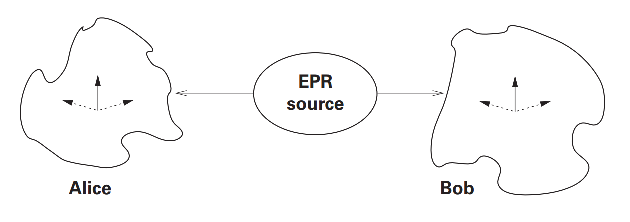
\includegraphics[scale=0.15]{figures/EPR}
    \caption{EPR}
  \end{figure}
  \end{columns}
  The special relativity; the speed of light; the symmetry of observers. \\
  Even though the results themselves are perfectly compatible with relativity theory, the behavior remains mysterious.
  But this mysterious behavior could also be explained by a classical theory that postulates that
  particles have an internal \textbf{hidden} state that determines the result of the measurement.

  \vspace{0.3cm}
  Let $O_{\theta}$ be a single-qubit Hermitian associated with two-subspace decomposition:
    $\{\ket{\mathbf{v}}\} \bigoplus \{\ket{\mathbf{v}^{\perp}}\}$
  \begin{align*}
    \ket{\mathbf{v}} &= \cos \theta \ket0 + \sin \theta \ket1 \\
    \ket{\mathbf{v}^{\perp}} &= -\sin \theta \ket0 + \cos \theta \ket1
  \end{align*}
  Let
  \begin{align*}
    O_{\theta_{1}} &\rightarrow \{\ket{\mathbf{v}_1}\} \bigoplus \{\ket{\mathbf{v}_1^{\perp}}\} \\
    O_{\theta_{2}} &\rightarrow \{\ket{\mathbf{v}_2}\} \bigoplus \{\ket{\mathbf{v}_2^{\perp}}\} \\
    P^{\mathbf{v}_1} &= \ket{\mathbf{v}_1} \bra{\mathbf{v}_1}
    \qquad
    P^{\mathbf{v}_1^{\perp}} = \ket{\mathbf{v}_1^{\perp}} \bra{\mathbf{v}_1^{\perp}}
    \\
    P^{\mathbf{v}_2} &= \ket{\mathbf{v}_2} \bra{\mathbf{v}_2}
    \qquad
    P^{\mathbf{v}_2^{\perp}} = \ket{\mathbf{v}_2^{\perp}} \bra{\mathbf{v}_2^{\perp}}
  \end{align*}
  }%
\end{frame}

\begin{frame}{EPR Paradox and Bell's Theorem - II\tiny{\cite{solutionofexercise420}}}
  {\tiny
    \begin{align*}
      P &= (P^{\mathbf{v}_1} \otimes I)(I \otimes P^{\mathbf{v}_2}) +
           (P^{\mathbf{v}_1^{\perp}} \otimes I) (I \otimes P^{\mathbf{v}_2^{\perp}}) \\
      &=
      (P^{\mathbf{v}_1} \otimes P^{\mathbf{v}_2}) +
      (P^{\mathbf{v}_1^{\perp}} \otimes P^{\mathbf{v}_2^{\perp}})
      \\
      P^{\mathbf{v}_1\mathbf{v}_2} &= P^{\mathbf{v}_1} \otimes P^{\mathbf{v}_2} \\
      &= (\ket{\mathbf{v}_1}\bra{\mathbf{v}_1}) \otimes (\ket{\mathbf{v}_2}\bra{\mathbf{v}_2}) \\
      &= (\ket{\mathbf{v}_1} \otimes \ket{\mathbf{v}_2}) \; (\bra{\mathbf{v}_1} \otimes \bra{\mathbf{v}_2}) \\
      &= (\ket{\mathbf{v}_1} \otimes \ket{\mathbf{v}_2}) \;
         [
           (\cos \theta_1 \cos \theta_2) \ket{00}
         + (\cos \theta_1 \sin \theta_2) \ket{01}
         + (\sin \theta_1 \cos \theta_2) \ket{10}
         + (\sin \theta_1 \sin \theta_2) \ket{11}
         ]
      \\
      P^{\mathbf{v}_1^{\perp} \mathbf{v}_2^{\perp}} &= 
         (\ket{\mathbf{v}_1^{\perp}} \otimes \ket{\mathbf{v}_2^{\perp}}) \;
         [
           (\sin \theta_1 \sin\theta_2) \ket{00}
         - (\sin \theta_1 \cos \theta_2) \ket{01}
         - (\cos \theta_1 \sin \theta_2) \ket{10}
         + (\cos \theta_1 \cos \theta_2) \ket{11}
         ]
      \\
      P\ket{\psi} &= P \frac{1}{\sqrt2} (\ket{00} + \ket{11}) \\
      &= \frac{1}{\sqrt2} 
                     [
                       (\ket{\mathbf{v}_1} \otimes \ket{\mathbf{v}_2}) (\cos \theta_1 \cos \theta_2 + \sin \theta_1 \sin \theta_2)
                     + (\ket{\mathbf{v}_1^{\perp}} \otimes \ket{\mathbf{v}_2^{\perp}}) (\sin \theta_1 \sin\theta_2 + \cos \theta_1 \cos \theta_2)
                     ] \\
      &= \frac{1}{\sqrt2} 
         [
           (\ket{\mathbf{v}_1} \otimes \ket{\mathbf{v}_2}) \cos (\theta_1 - \theta_2) 
         + (\ket{\mathbf{v}_1^{\perp}} \otimes \ket{\mathbf{v}_2^{\perp}}) \cos (\theta_1 - \theta_2)
         ] \\
      &= \frac{1}{\sqrt2} \cos (\theta_1 - \theta_2)
         [
           \ket{\mathbf{v}_1} \otimes \ket{\mathbf{v}_2}
         + \ket{\mathbf{v}_1^{\perp}} \otimes \ket{\mathbf{v}_2^{\perp}}
         ]
      \\
      p = \braket{\psi|P|\psi}
      &= \frac{1}{2} \cos (\theta_1 - \theta_2) [ \bra{00} \ket{\mathbf{v_1}} \ket{\mathbf{v}_2}
                                                + \bra{00} \ket{\mathbf{v}_1^{\perp}} \ket{\mathbf{v}_2^{\perp}}
                                                + \bra{11} \ket{\mathbf{v}_1} \ket{\mathbf{v}_2}
                                                + \bra{11} \ket{\mathbf{v}_1^{\perp}} \ket{\mathbf{v}_2^{\perp}}
                                                ] \\
      &= \frac{1}{2} \cos (\theta_1 - \theta_2) [ \cos \theta_1 \cos \theta_2
                                                + \sin \theta_1 \sin \theta_2
                                                + \sin \theta_1 \sin \theta_2
                                                + \cos \theta_1 \cos \theta_2
                                                ] \\
      &= \cos^2 (\theta_1 - \theta_2)
    \end{align*}
  }%
\end{frame}

\begin{frame}{EPR Paradox and Bell's Theorem - III}
  {\tiny
    If the polaroids are set randomly for a series of EPR pairs emanating from the source, then
    \begin{enumerate}[I]
    \item with probability $1/3$ the polaroid orientation will be the same and the measurements will agree,
    \item with probability $2/3$ the polaroid orientation will differ and the measurements will agree with probability $1/4$.
    \end{enumerate}
  }%
  Thus, overall, the measurements will agree half the time and disagree half the time. When such
  an experiment is performed, these are indeed the probabilities that are seen.
\end{frame}

\begin{frame}{EPR Paradox and Bell's Theorem - IV}
  {\tiny
  \begin{table}[h!]
  \begin{center}
    \caption{Hidden Variable}
    \label{tab:table1}
    \begin{tabular}{c|c|c|c|c|c|c|c|c}
                          & $\mathbf{h}_0$                & $\mathbf{h}_1$                & $\mathbf{h}_2$                & $\mathbf{h}_3$                & $\mathbf{h}_4$                & $\mathbf{h}_5$                & $\mathbf{h}_6$                & $\mathbf{h}_7$ \\
                          & $\nearrow  \uparrow \nwarrow$ & $\nearrow  \uparrow \nwarrow$ & $\nearrow  \uparrow \nwarrow$ & $\nearrow  \uparrow \nwarrow$ & $\nearrow  \uparrow \nwarrow$ & $\nearrow  \uparrow \nwarrow$ & $\nearrow  \uparrow \nwarrow$ & $\nearrow  \uparrow \nwarrow$ \\
        Polaroids Setting & P          P        P         & P          P        A         & P          A        P         & P          A        A         & A          P        P         & A          P        A         & A          A        P         & A          A        A         \\
      \hline
      $\nwarrow \nwarrow$ & P          P                  & A          A                  & P          P                  & A          A                  & P          P                  & A          A                  & P          P                  & A          A                  \\
      $\nwarrow \uparrow$ & P          P                  & A          P                  & P          A                  & A          A                  & P          P                  & A          P                  & P          A                  & A          A                  \\
      $\nwarrow \nearrow$ & P          P                  & A          P                  & P          P                  & A          P                  & P          A                  & A          A                  & P          A                  & A          A                  \\
      $\uparrow \nwarrow$ & P          P                  & P          A                  & A          P                  & A          A                  & P          P                  & P          A                  & A          P                  & A          A                  \\
      $\uparrow \uparrow$ & P          P                  & P          P                  & A          A                  & A          A                  & P          P                  & P          P                  & A          A                  & A          A                  \\
      $\uparrow \nearrow$ & P          P                  & P          P                  & A          P                  & A          P                  & P          A                  & P          A                  & A          A                  & A          A                  \\
      $\nearrow \nwarrow$ & P          P                  & P          A                  & P          P                  & P          A                  & A          P                  & A          A                  & A          P                  & A          A                  \\
      $\nearrow \uparrow$ & P          P                  & P          P                  & P          A                  & P          A                  & A          P                  & A          P                  & A          A                  & A          A                  \\
      $\nearrow \nearrow$ & P          P                  & P          P                  & P          P                  & P          P                  & A          A                  & A          A                  & A          A                  & A          A                  \\
      \hline
     Possibility of Agree & $1$                           & $5/9$                         & $5/9$                         & $5/9$                         & $5/9$                         & $5/9$                         & $5/9$                         & $1$                           \\
    \end{tabular}
  \end{center}
  \end{table}
  }%
\end{frame}

\section{Quantum State Transformations}
\begin{frame}
  Quantum State Transformations
\end{frame}

\subsection{Unitary Transformations}
\begin{frame}{Quantum Transformation}
  {\tiny
    Quantum Transformation means a mapping from the state space of a quantum system to itself.
    While for measurements, there are only finite outcomes, and the results are only probabilistic.\\
    The quantum properties of the quantum system will be respected after a transformation.
    The result of a measurement is deterministic without any quantum properties being kept.\\
    A quantum state transformation is \textbf{reversible}, while a measurement not.\\
    Transformation and measurement exist in Nature. What's the relation between them exactly?\\
    \vspace{0.3cm}
    In sense of math, measurement is modeled as a projector matrix (subspace decomposition), i.e. $P\ket{\psi}$;
    now transformation is modeled as a matrix called unitary $U$ with property $U^{\dagger}U = I$, i.e. $U\ket{\psi}$\\
    The unitarity condition simply ensures that the transformation does not violate any general principles of quantum theory.
    Geometrically, all quantum state transformations are rotations of the complex vector space associated with the quantum state space.
    \begin{align*}
      U^TU &=
        \begin{bmatrix}
          \mathbf{u}_1^T \\
          \mathbf{u}_2^T \\
          \mathbf{u}_3^T
        \end{bmatrix}
        \begin{bmatrix} \mathbf{u}_1 \mathbf{u}_2 \mathbf{u}_3 \end{bmatrix} 
        = 
        \begin{bmatrix}
          \mathbf{u}_1^T \mathbf{u}_1 & \mathbf{u}_1^T \mathbf{u}_2 & \mathbf{u}_1^T \mathbf{u}_3 \\
          \mathbf{u}_2^T \mathbf{u}_1 & \mathbf{u}_2^T \mathbf{u}_2 & \mathbf{u}_2^T \mathbf{u}_3 \\
          \mathbf{u}_3^T \mathbf{u}_1 & \mathbf{u}_3^T \mathbf{u}_2 & \mathbf{u}_3^T \mathbf{u}_3
        \end{bmatrix}
    \end{align*}
    \vspace{0.3cm}
    The product $U_1 U_2$ of two unitary transformations is again unitary. \\
    The tensor product $U_1 \otimes U_2$ is a unitary transformation of the space $X_1 \otimes X_2$ if $U_1$ and $U_2$ are unitary transformations of $X_1$ and $X_2$ respectively.\\
    Linear combinations of unitary operators, however, are not in general unitary.
  }%
\end{frame}

\begin{frame}{The No-Cloning Principle}
  {\tiny
    Suppose $U$ is a unitary transformation that clones: $U\ket{a}\ket{0} = \ket{a}\ket{a}$, by linearity,
    \begin{align*}
      \ket{c} &= \frac{1}{\sqrt2} (\ket{a} + \ket{b}) \\
      U\ket{c}\ket{0} &=  \frac{1}{\sqrt2} ( \ket{a}\ket{a} + \ket{b}\ket{b} ) \\
                      &=  \ket{c}\ket{c} = \frac{1}{2} (  \ket{a}\ket{a} + \ket{a}\ket{b} + \ket{b}\ket{a} + \ket{b}\ket{b} )
    \end{align*}
    Thus, there is no unitary operation that can reliably clone \textbf{all} quantum states.
    The no-cloning theorem tells us that it is impossible to clone a specific unknown quantum state reliably.
    It does not preclude the construction of a known quantum state from a known quantum state.
  }%
\end{frame}

\subsection{Some Simple Quantum Transformations/Gates}

\begin{frame}{The Pauli Transformations}
  {\tiny
    \begin{align*}
      I &= \ket0\bra0 + \ket1\bra1 = \begin{bmatrix} 1 & 0 \\ 0 & 1 \end{bmatrix} \\
      X &= \ket1\bra0 + \ket0\bra1 = \begin{bmatrix} 0 & 1 \\ 1 & 0 \end{bmatrix} \\
      Y &= -\ket1\bra0 + \ket0\bra1 = \begin{bmatrix} 0 & 1 \\ -1 & 0 \end{bmatrix} \\
      Z &= \ket0\bra0 - \ket1\bra1 = \begin{bmatrix} 1 & 0 \\ 0 & -1 \end{bmatrix} \\
      Y &= ZX \\
      Y' &= -iY = \begin{bmatrix} 0 & -i \\ i & 0 \end{bmatrix} \\
      \mathbf{X}^2 &= \mathbf{Y'}^2 = \mathbf{Z}^2 = -i\mathbf{XY'Z} = \mathbf{I} \\
      \mathbf{XY'} &= -\mathbf{Y'X} = i\mathbf{Z} \\
      \mathbf{Y'Z} &= -\mathbf{ZY'} = i\mathbf{X} \\
      \mathbf{ZX} &= -\mathbf{XZ} = i\mathbf{Y'}
    \end{align*}
  }%
\end{frame}

\begin{frame}{The Hadamard Transformation}
  {\tiny
    \begin{align*}
      H &= \frac{1}{\sqrt2}(\ket0\bra0 + \ket1\bra0 + \ket0\bra1 -\ket1\bra1) \\
        &= \frac{1}{\sqrt2} \begin{bmatrix} 1 & 1 \\ 1 & -1 \end{bmatrix} \\
      H\ket0 &= \ket+ = \frac{1}{\sqrt2} (\ket0 + \ket1) \\
      H\ket1 &= \ket- = \frac{1}{\sqrt2} (\ket0 - \ket1) \\
      HH &= I
    \end{align*}
    The graphical representation:
    % definitions for the circuit elements
    \def\gAxA{\op{H}\w\A{gAxA}}
    
    % definitions for bit labels and initial states
    \def\bA{ \q{q_{0}}}
    
    \begin{align*}
    % The quantum circuit as an xymatrix
    \xymatrix@R=5pt@C=10pt{
            & \gAxA &\n
    }
    \end{align*}
  }%
\end{frame}

\begin{frame}{The Controlled-NOT - I}
  {\tiny
    \begin{align*}
      \ket0\bra0 \otimes \ket1\bra1 &= \begin{bmatrix} 1 & 0 \\ 0 & 0 \end{bmatrix} \otimes \begin{bmatrix} 0 & 0 \\ 0 & 1 \end{bmatrix} \\
      \ket{01}\bra{01}
      &= \begin{bmatrix} 0 \\ 1 \\ 0 \\ 1 \end{bmatrix} \begin{bmatrix} 0 & 1 & 0 & 0\end{bmatrix} 
       = \begin{bmatrix} 0 & 0 & 0 & 0 \\ 0 & 1 & 0 & 0 \\ 0 & 0 & 0 & 0 \\ 0 & 0 & 0 & 0 \end{bmatrix} \\
      \ket1\bra1 \otimes \ket1\bra0 &= \begin{bmatrix} 0 & 0 \\ 0 & 1 \end{bmatrix} \otimes \begin{bmatrix} 0 & 0 \\ 1 & 0 \end{bmatrix} \\
      \ket{11}\bra{10}
      &= \begin{bmatrix} 0 \\ 0 \\ 0 \\ 1 \end{bmatrix} \begin{bmatrix} 0 & 0 & 1 & 0\end{bmatrix} 
       = \begin{bmatrix} 0 & 0 & 0 & 0 \\ 0 & 0 & 0 & 0 \\ 0 & 0 & 0 & 0 \\ 0 & 0 & 1 & 0 \end{bmatrix} \\
    \end{align*}
    \begin{align*}
      C_{not} &= \ket0\bra0 \otimes I + \ket1\bra1 \otimes \mathbf{X} \\
              &= \ket0\bra0 \otimes (\ket0\bra0 +\ket1\bra1) + \ket1\bra1 \otimes (\ket1\bra0 + \ket0\bra1) \\
              &= \ket{00}\bra{00} + \ket{01}\bra{01} + \ket{11}\bra{10} + \ket{10}\bra{11} \\
              &= \begin{bmatrix} 1 & 0 & 0 & 0 \\ 0 & 1 & 0 & 0 \\ 0 & 0 & 0 & 1 \\ 0 & 0 & 1 & 0 \end{bmatrix} 
              = \begin{bmatrix} I & 0 \\ 0 & X \end{bmatrix} \\
      C_{not}C_{not} &= I
    \end{align*}
  }%
\end{frame}

\begin{frame}{The Controlled-NOT - II}
  {\tiny
    \begin{align*}
      C_{not}\ket{00} &= \ket{00} \\
      C_{not}\ket{01} &= \ket{01} \\
      C_{not}\ket{10} &= \ket{11} \\
      C_{not}\ket{11} &= \ket{10}
    \end{align*}
    \begin{align*}
      \ket\psi &= \frac{1}{\sqrt2} (\ket0 + \ket1) \otimes \ket0 = \frac{1}{\sqrt2} (\ket0 \otimes \ket0 + \ket1 \otimes \ket0) \\
      &= \frac{1}{\sqrt2} (\begin{bmatrix} 1 \\ 0 \\ 0 \\ 0 \end{bmatrix}  + \begin{bmatrix} 0 \\ 0 \\ 1 \\ 0 \end{bmatrix})
       = \frac{1}{\sqrt2} \begin{bmatrix} 1 \\ 0 \\ 1 \\ 0 \end{bmatrix} \\
      C_{not}\ket\psi &=
      \frac{1}{\sqrt2} \begin{bmatrix} 1 & 0 & 0 & 0 \\ 0 & 1 & 0 & 0 \\ 0 & 0 & 0 & 1 \\ 0 & 0 & 1 & 0 \end{bmatrix}  
                       \begin{bmatrix} 1 \\ 0 \\ 1 \\ 0 \end{bmatrix}
      = \frac{1}{\sqrt2} \begin{bmatrix} 1 \\ 0 \\ 0 \\ 1 \end{bmatrix}
      = \frac{1}{\sqrt2} (\begin{bmatrix} 1 \\ 0 \\ 0 \\ 0 \end{bmatrix} + \begin{bmatrix} 0 \\ 0 \\ 0 \\ 1 \end{bmatrix}) \\
      &= \frac{1}{\sqrt2}(\ket{00} + \ket{11})
    \end{align*}
    The $C_{not}$ can be represented as a gate in graphical form:
    \begin{align*}
    % definitions for the circuit elements
    \def\gAxA{\b\w\A{gAxA}}
    \def\gAxB{\op{X}\w\A{gAxB}}
    % definitions for bit labels and initial states
    \def\bA{ \q{q_{0}}}
    \def\bB{ \q{q_{1}}}
    % The quantum circuit as an xymatrix
    \xymatrix@R=5pt@C=10pt{
        \bA & \gAxA &\n
    \\  \bB & \gAxB &\n
    % Vertical lines and other post-xymatrix latex
    \ar@{-}"gAxB";"gAxA"
    }
    \end{align*}
  }%
\end{frame}

\begin{frame}{The Controlled-NOT - III}
  {\tiny
    \begin{align*}
      % definitions for the circuit elements
      \def\gAxA{\op{X}\w\A{gAxA}}
      \def\gBxA{\b\w\A{gBxA}}
      \def\gBxB{\op{X}\w\A{gBxB}}
      \def\gCxA{\op{X}\w\A{gCxA}}
      % definitions for bit labels and initial states
      \def\bA{ \q{q_{0}}}
      \def\bB{ \q{q_{1}}}
      % The quantum circuit as an xymatrix
      \xymatrix@R=5pt@C=10pt{
          \bA & \gAxA &\gBxA &\gCxA &\n
      \\  \bB & \n   &\gBxB &\n   &\n
      % Vertical lines and other post-xymatrix latex
      \ar@{-}"gBxB";"gBxA" \\
      }
    \end{align*}
    This circuit represents transformation: $(X \otimes I) \begin{bmatrix} I & 0 \\ 0 & X \end{bmatrix} (X \otimes I)$ \\
    Given
    \begin{align*}
      X \otimes I &= \begin{bmatrix} 0 & 1 \\ 1 & 0 \end{bmatrix} \otimes \begin{bmatrix} 1 & 0 \\ 0 & 1 \end{bmatrix}
      =\begin{bmatrix}
        0 & 0 & 1 & 0 \\
        0 & 0 & 0 & 1 \\
        1 & 0 & 0 & 0 \\
        0 & 1 & 0 & 0
       \end{bmatrix}
    \end{align*}
    The transformation is:
    \begin{align*}
        &\begin{bmatrix}
        0 & 0 & 1 & 0 \\
        0 & 0 & 0 & 1 \\
        1 & 0 & 0 & 0 \\
        0 & 1 & 0 & 0
        \end{bmatrix}
        \begin{bmatrix}
        1 & 0 & 0 & 0 \\
        0 & 1 & 0 & 0 \\
        0 & 0 & 0 & 1 \\
        0 & 0 & 1 & 0
        \end{bmatrix}
        \begin{bmatrix}
        0 & 0 & 1 & 0 \\
        0 & 0 & 0 & 1 \\
        1 & 0 & 0 & 0 \\
        0 & 1 & 0 & 0
        \end{bmatrix} \\
        = &
        \begin{bmatrix}
        0 & 0 & 1 & 0 \\
        0 & 0 & 0 & 1 \\
        1 & 0 & 0 & 0 \\
        0 & 1 & 0 & 0
        \end{bmatrix}
        \begin{bmatrix}
        0 & 0 & 1 & 0 \\
        0 & 0 & 0 & 1 \\
        0 & 1 & 0 & 0 \\
        1 & 0 & 0 & 0
        \end{bmatrix} \\
        = &
        \begin{bmatrix}
        0 & 1 & 0 & 0 \\
        1 & 0 & 0 & 0 \\
        0 & 0 & 1 & 0 \\
        0 & 0 & 0 & 1
        \end{bmatrix}
        = \begin{bmatrix} X & 0 \\ 0 & I \end{bmatrix}
    \end{align*}
  }%
\end{frame}

\begin{frame}{Some Simple Gates}
  {\tiny
    \begin{align*}
      C_{not} &= \ket0\bra0 \otimes I + \ket1\bra1 \otimes \mathbf{X} = \begin{bmatrix} I & 0 \\ 0 & X \end{bmatrix} \\
      \Lambda Q &= \ket0\bra0 \otimes I + \ket1\bra1 \otimes \mathbf{Q} = \begin{bmatrix} I & 0 \\ 0 & Q \end{bmatrix} \\
      \Lambda X &= C_{not}
    \end{align*}

    The swap circuit:
    % definitions for the circuit elements
    \def\gAxA{\b\w\A{gAxA}}
    \def\gAxB{\o\w\A{gAxB}}
    \def\gBxB{\b\w\A{gBxB}}
    \def\gBxA{\o\w\A{gBxA}}
    \def\gCxA{\b\w\A{gCxA}}
    \def\gCxB{\o\w\A{gCxB}}
    
    % definitions for bit labels and initial states
    \def\bA{ \q{q_{0}}}
    \def\bB{ \q{q_{1}}}
    
    \begin{align*}
    % The quantum circuit as an xymatrix
    \xymatrix@R=5pt@C=10pt{
        \bA & \gAxA &\gBxA &\gCxA &\n
    \\  \bB & \gAxB &\gBxB &\gCxB &\n
    %
    % Vertical lines and other post-xymatrix latex
    %
    \ar@{-}"gAxB";"gAxA"
    \ar@{-}"gBxA";"gBxB"
    \ar@{-}"gCxB";"gCxA"
    }
    \end{align*}

    $C_{not}$ in Hadamard basis (We have not changed the transformation at all, only the way we are thinking about it):
    \begin{align*}
      C_{not}\ket{++} &= \ket{++} \\
      C_{not}\ket{+-} &= \ket{--} \\
      C_{not}\ket{-+} &= \ket{-+} \\
      C_{not}\ket{--} &= \ket{+-}
    \end{align*}

    Following two gates are same actually:
    % definitions for the circuit elements
    \def\gAxA{\op{H}\w\A{gAxA}}
    \def\gAxB{\op{H}\w\A{gAxB}}
    \def\gBxA{\b\w\A{gBxA}}
    \def\gBxB{\o\w\A{gBxB}}
    \def\gCxA{\op{H}\w\A{gCxA}}
    \def\gCxB{\op{H}\w\A{gCxB}}
    \def\gDxA{\b\w\A{gDxA}}
    \def\gDxB{\o\w\A{gDxB}}
    
    % definitions for bit labels and initial states
    
    \def\bA{ \q{q_{0}}}
    \def\bB{ \q{q_{1}}}
    
    \begin{align*}
    % The quantum circuit as an xymatrix
    \xymatrix@R=7pt@C=21pt{
            & \gAxA &\gBxA &\gCxA &\n & & \gDxB &\n 
    \\      & \gAxB &\gBxB &\gCxB &\n & & \gDxA &\n
    %
    % Vertical lines and other post-xymatrix latex
    %
    \ar@{-}"gBxB";"gBxA"
    \ar@{-}"gDxB";"gDxA"
    }
    \end{align*}
  }%
\end{frame}

\begin{frame}{Dense Coding}
    {\tiny
    Alice wants to send 2 bits to Bob with help of a EPR $\ket{\psi} = \frac{1}{\sqrt2} (\ket{00} + \ket{11} )$
    }%
    \begin{figure}
      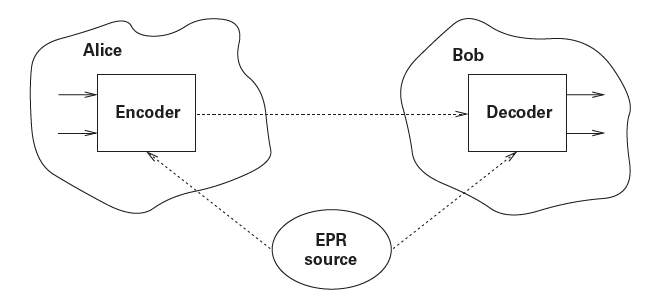
\includegraphics[scale=0.15]{figures/dense-coding}
      \caption{Dense Coding}
    \end{figure}
    \begin{columns}[t]
    \column{0.5\textwidth}
    {\tiny
    Alice encodes 2 bits with $q_0$ and sends the qubit to Bob:
    \begin{align*}
      \ket{\psi_0} &= (I \otimes I) \ket{\psi} = \frac{1}{\sqrt2} (\ket{00} + \ket{11} ) \\
      \ket{\psi_1} &= (X \otimes I) \ket{\psi} = \frac{1}{\sqrt2} (\ket{10} + \ket{01} ) \\
      \ket{\psi_2} &= (Z \otimes I) \ket{\psi} = \frac{1}{\sqrt2} (\ket{00} - \ket{11} ) \\
      \ket{\psi_3} &= (Y \otimes I) \ket{\psi} = \frac{1}{\sqrt2} (\ket{01} - \ket{10} )
    \end{align*}
    }%
    \column{0.5\textwidth}
    {\tiny
    % definitions for the circuit elements
    \def\gAxA{\b\w\A{gAxA}}
    \def\gAxB{\o\w\A{gAxB}}
    \def\gBxA{\op{H}\w\A{gBxA}}
    % definitions for bit labels and initial states
    \def\bA{ \q{q_{0}}}
    \def\bB{ \q{q_{1}}}
    % The quantum circuit as an xymatrix
    Bob decodes the qubit with gates:
    \begin{align*}
    \xymatrix@R=5pt@C=10pt{
        \bA & \gAxA &\gBxA &\n
    \\  \bB & \gAxB &\n   &\n
    % Vertical lines and other post-xymatrix latex
    \ar@{-}"gAxB";"gAxA"
    }
    \end{align*}
    \begin{align*}
      (H \otimes I) C_{not} \ket{\psi_0} &= (H \otimes I)\frac{1}{\sqrt2} (\ket{00} + \ket{10} ) = \ket{00} \\
      (H \otimes I) C_{not} \ket{\psi_1} &= (H \otimes I)\frac{1}{\sqrt2} (\ket{11} + \ket{01} ) = \ket{01} \\
      (H \otimes I) C_{not} \ket{\psi_2} &= (H \otimes I)\frac{1}{\sqrt2} (\ket{00} - \ket{10} ) = \ket{10} \\
      (H \otimes I) C_{not} \ket{\psi_3} &= (H \otimes I)\frac{1}{\sqrt2} (\ket{01} - \ket{11} ) = \ket{11}
    \end{align*}
    }%
    \end{columns}
\end{frame}

\begin{frame}{Teleportation}
  {\tiny
  Alice wants to send $\ket{\phi} = a \ket{0} + b\ket{1}$ to Bob with help of a EPR $\ket{\psi} = \frac{1}{\sqrt2} (\ket{00} + \ket{11} )$.
  }%
  \begin{figure}
    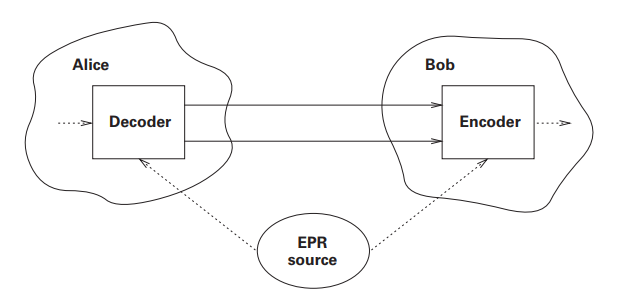
\includegraphics[scale=0.15]{figures/teleporation}
    \caption{Teleportation}
  \end{figure}
  \begin{columns}[t]
  \column{0.5\textwidth}
  {\tiny
  Alice transforms the 2 qubits she holds and then sends the result of measurement to Bob.
  \begin{align*}
    & ( H \otimes I \otimes I ) ( C_{not} \otimes I ) ( \ket{\phi} \otimes \ket{\psi} ) \\
    &= ( H \otimes I \otimes I ) ( C_{not} \otimes I ) \\
    &  \qquad \frac{1}{\sqrt2} ( a \ket{000} + a \ket{011} + b \ket{100} + b \ket{111} ) \\
    &= ( H \otimes I \otimes I ) \frac{1}{\sqrt2} ( a \ket{000} + a \ket{011} + b \ket{110} + b \ket{101} ) \\
    &= \frac{1}{2} ( a \ket{000} + a \ket{100} + a \ket{011} + a \ket{111} + \\
    &  \quad \qquad   b \ket{010} - b \ket{110} + b \ket{001} - b \ket{101}) \\
    &= \frac{1}{2} ( \ket{00} (a\ket0 + b\ket1) + \ket{01} ( a \ket1 + b \ket0) \\
    &  \quad \qquad  \ket{10} (a\ket0 - b\ket1) + \ket{11} ( a \ket1 - b \ket0)
  \end{align*}
  }%
  \column{0.5\textwidth}
  {\tiny
  Bob transforms the qubit he holds based on the bits he received:
  \begin{align*}
    00&: I (a\ket0 + b\ket1) = a\ket0 + b\ket1 \\
    01&: X (a\ket1 + b\ket0) = a\ket0 + b\ket1 \\
    10&: Z (a\ket0 - b\ket1) = a\ket0 + b\ket1 \\
    11&: Y (a\ket1 - b\ket0) = a\ket0 + b\ket1
  \end{align*}
  }%
  \end{columns}
\end{frame}

\begin{frame}{Bloch Sphere of Single Qubit and Rotations}
  {\tiny
    $\ket{\psi} = \cos(\frac{\theta}2)\ket{0}+e^{i\phi}\sin(\frac{\theta}2)\ket{1}$, where $0\leqslant\theta\leqslant\pi$, $0\leqslant\phi\leqslant2\pi$.
    \begin{figure}
      \centering
      \begin{subfigure}[b]{0.5\textwidth}
        \centering
        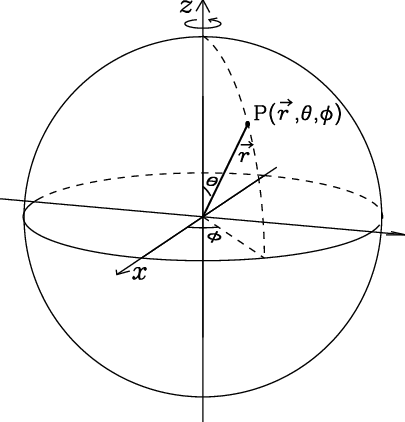
\includegraphics[scale=0.1]{figures/The-spherical-polar-coordinate-system}
        \caption{The spherical polar coordinate system\tiny\cite{sphericalpolarcoordinate}}
      \end{subfigure}
      \hfill
      \begin{subfigure}[b]{0.5\textwidth}
        \centering
        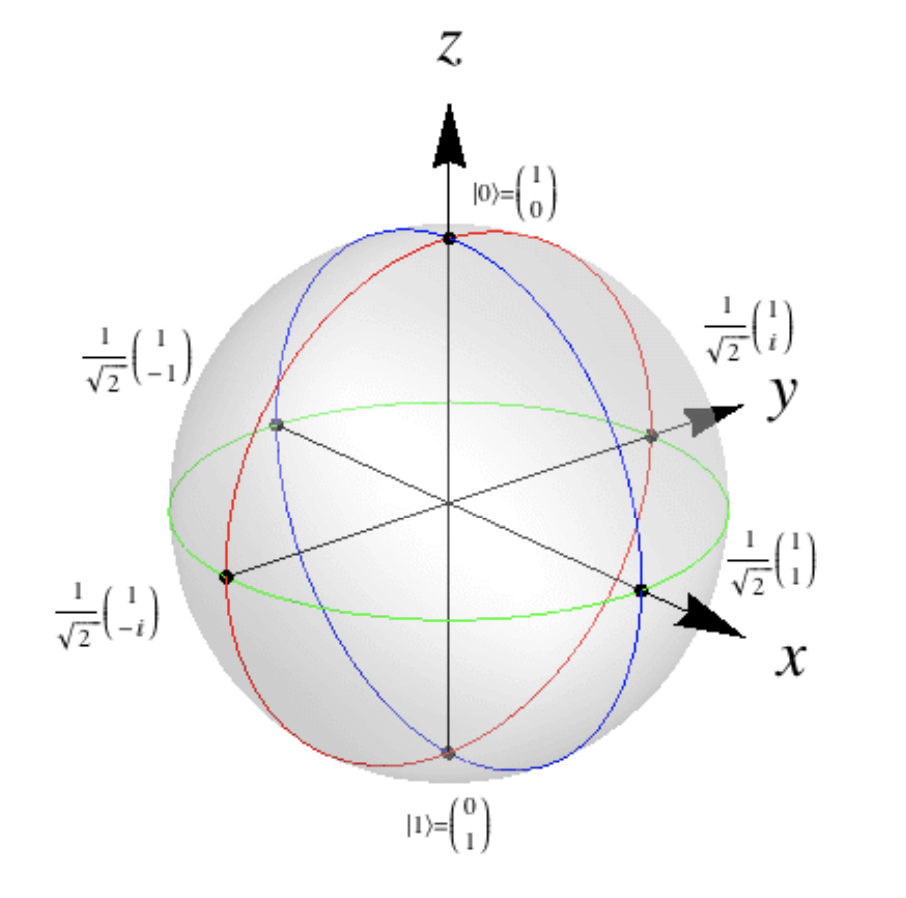
\includegraphics[scale=0.12]{figures/singlequbitstates}
        \caption{The special single qubit states\tiny\cite{singlequbitstates}}
      \end{subfigure}
      \caption{The Block Sphere}
    \end{figure}
    Defined operators $R_x(\alpha)$, $R_y(\alpha)$ and $R_z(\alpha)$:
    \begin{align*}
      R_x(\alpha) &\equiv \cos\frac{\alpha}2\mathbf{I} - i\sin\frac{\alpha}2
                                                                     \begin{bmatrix}
                                                                       1 & 0 \\
                                                                       0 & 1
                                                                     \end{bmatrix}
                  &= e^{-i\frac{\alpha}2\mathbf{X}}
                  &= \cos\frac{\alpha}2\mathbf{I} - i\sin\frac{\alpha}2 \mathbf{X}
                  &&=\begin{bmatrix}
                    \cos\frac{\alpha}2 & -i\sin\frac{\alpha}2 \\
                    -i\sin\frac{\alpha}2 & \cos\frac{\alpha}2
                    \end{bmatrix} \\
      R_y(\alpha) &\equiv \cos\frac{\alpha}2\mathbf{I} - i\sin\frac{\alpha}2
                                                                     \begin{bmatrix}
                                                                       0 & -i \\
                                                                       i & 0
                                                                     \end{bmatrix}
                  &= e^{-i\frac{\alpha}2\mathbf{Y}}
                  &= \cos\frac{\alpha}2\mathbf{I} - i\sin\frac{\alpha}2 \mathbf{Y}
                  &&=\begin{bmatrix}
                    \cos\frac{\alpha}2 & -\sin\frac{\alpha}2 \\
                    \sin\frac{\alpha}2 & \cos\frac{\alpha}2
                    \end{bmatrix} \\
      R_z(\alpha) &\equiv \cos\frac{\alpha}2\mathbf{I} - i\sin\frac{\alpha}2
                                                                     \begin{bmatrix}
                                                                       1 & 0 \\
                                                                       0 & -1
                                                                     \end{bmatrix}
                  &= e^{-i\frac{\alpha}2\mathbf{Z}}
                  &= \cos\frac{\alpha}2\mathbf{I} - i\sin\frac{\alpha}2 \mathbf{Z}
                  &&=\begin{bmatrix}
                    e^{-i\frac{\alpha}2} & 0 \\
                    0 & e^{i\frac{\alpha}2}
                    \end{bmatrix} \\
    \end{align*}
  }%
\end{frame}

\begin{frame}{A Set of Primitive Transformations}
  {\tiny
    Define transformations:
    \begin{align*}
      K(\delta) &= e^{i\delta}I & \mbox{A phase shift} \\
      R(\beta)  &= \begin{bmatrix} \cos\beta & \sin\beta \\ -\sin\beta & \cos\beta \end{bmatrix}  & \mbox{A rotation $2\beta$ (left-hand) about the y-axis} \\
      T(\alpha) &= \begin{bmatrix} e^{i\alpha} & 0 \\ 0 & e^{-i\alpha} \end{bmatrix} & \mbox{A rotation $2\alpha$ (left-hand) about the z-axis} \\
    \end{align*}
    \begin{align*}
      &R(\beta)R(-\beta) = I, T(\alpha)T(-\alpha) = I \\
      &XR(\beta)X = R(-\beta), XT(\alpha)X = T(-\alpha) \\
      &T(\alpha)T(\gamma) = T(\alpha + \gamma)
    \end{align*}
    Any single-qubit transformation $Q$ can be decomposed into a sequence of transformations of the form
    \begin{align*}
      K(\delta)T(\alpha)R(\beta)T(\gamma) =
       \begin{bmatrix}
          e^{i(\delta + \alpha + \gamma)} \cos\beta & e^{i(\delta + \alpha - \gamma)} \sin\beta \\
         -e^{i(\delta - \alpha + \gamma)} \sin\beta & e^{i(\delta - \alpha - \gamma)} \cos\beta
       \end{bmatrix}.
    \end{align*}
    Given the transformation $Q$, it follows immediately from the unitary condition $QQ^{\dagger}=I$.
    And indeed:
    \begin{align*}
      \begin{bmatrix}
         e^{i(\delta + \alpha + \gamma)} \cos\beta & e^{i(\delta + \alpha - \gamma)} \sin\beta \\
        -e^{i(\delta - \alpha + \gamma)} \sin\beta & e^{i(\delta - \alpha - \gamma)} \cos\beta
      \end{bmatrix}
      \begin{bmatrix}
        e^{-i(\delta + \alpha + \gamma)} \cos\beta & -e^{-i(\delta - \alpha + \gamma)} \sin\beta \\
        e^{-i(\delta + \alpha - \gamma)} \sin\beta &  e^{-i(\delta - \alpha - \gamma)} \cos\beta
      \end{bmatrix} = I
    \end{align*}
  }%
\end{frame}


\begin{frame}{Examples of Primitive Transformations}
  {\tiny
    \begin{align*}
      K(\delta)T(\alpha)R(\beta)T(\gamma) =
       \begin{bmatrix}
          e^{i(\delta + \alpha + \gamma)} \cos\beta & e^{i(\delta + \alpha - \gamma)} \sin\beta \\
         -e^{i(\delta - \alpha + \gamma)} \sin\beta & e^{i(\delta - \alpha - \gamma)} \cos\beta
       \end{bmatrix}
    \end{align*}
    \begin{align*}
      Q &= K(\delta)T(\alpha)R(\beta)T(\gamma) \\
      I &= K(0) T(0) R(0) T(0) \\
      X &= K(-\frac{\pi}{2}) T(\frac{\pi}{2}) R(\frac{\pi}{2}) T(0) \\
      H &= K(-\frac{\pi}{2}) T(\frac{\pi}{2}) R(\frac{\pi}{4}) T(0) = \frac{1}{\sqrt{2}}\begin{bmatrix} 1 & 1 \\ 1 & -1\end{bmatrix}
    \end{align*}
  }%
\end{frame}

\begin{frame}{Decomposition of Single-Controlled-Not - I}
  {\tiny
    Let $Q=K(\delta)T(\alpha)R(\beta)T(\gamma)$, then:
    \begin{align*}
      \Lambda Q &= (\Lambda K(\delta)) (\Lambda (T(\alpha)R(\beta)T(\gamma))) \\
               &= (\Lambda K(\delta)) (\Lambda Q')
    \end{align*}
    \begin{align*}
      \Lambda K(\delta) &= \ket0 \bra0 \otimes I + \ket1 \bra1 K(\delta)
       = \ket0 \bra0 \otimes I + e^{i\delta}\ket1 \bra1 I \\
      &= (\begin{bmatrix} 1 & 0 \\ 0 & 0 \end{bmatrix} + e^{i\delta} \begin{bmatrix} 0 & 0 \\ 0 & 1 \end{bmatrix}) \otimes I
       = (\begin{bmatrix} e^{i\frac{\delta}{2}} & 0 \\ 0 & e^{i\frac{\delta}{2}}\end{bmatrix}
         + e^{i\delta} \begin{bmatrix} e^{-i\frac{\delta}{2}} & 0 \\ 0 & e^{i\frac{\delta}{2}} \end{bmatrix}) \otimes I \\
      &= (K(\frac{\delta}{2})T(-\frac{\delta}{2})) \otimes I
    \end{align*}
    Graphically,
    \begin{align*}
    % definitions for the circuit elements
    \def\gAxA{\b\w\A{gAxA}}
    \def\gAxB{\op{K(\delta)}\w\A{gAxB}}
    \def\gBxA{\op{T(-\frac{\delta}{2})}\w\A{gBxA}}
    \def\gCxA{\op{K(\frac{\delta}{2})}\w\A{gCxA}}
    % definitions for bit labels and initial states
    \def\bA{ \q{q_{0}}}
    \def\bB{ \q{q_{1}}}
    % The quantum circuit as an xymatrix
    \xymatrix@R=5pt@C=10pt{
        \bA & \gAxA &\n & &\gBxA &\gCxA &\n
    \\  \bB & \gAxB &\n & &\n    &\n    &\n
    % Vertical lines and other post-xymatrix latex
    \ar@{-}"gAxB";"gAxA"
    }
    \end{align*}
  }%
\end{frame}
    
\begin{frame}{Decomposition of Single-Controlled-Not - II}
  {\tiny
    Define:
    \begin{align*}
      Q_0 &= T(\alpha)R(\frac{\beta}{2}), \\
      Q_1 &= R(-\frac{\beta}{2})T(\frac{-\gamma - \alpha}{2}), \\
      Q_2 &= T(\frac{\gamma - \alpha}{2}).
    \end{align*}
    Following hold:
    \begin{align*}
      Q_0 Q_1 Q_2 &= T(\alpha)R(\frac{\beta}{2}) R(-\frac{\beta}{2})T(\frac{-\gamma - \alpha}{2}) T(\frac{\gamma - \alpha}{2}) = I \\
      Q_0 X Q_1 X Q_2 &=
      T(\alpha)R(\frac{\beta}{2}) X R(-\frac{\beta}{2}) X X T(\frac{-\gamma - \alpha}{2}) X T(\frac{\gamma - \alpha}{2}) \\
      &= T(\alpha) R(\beta) T(\gamma) = Q'
    \end{align*}
    A circuit is constructed as:
    \begin{align*}
    % definitions for the circuit elements
    \def\gAxB{\op{Q_2}\w\A{gAxB}}
    \def\gBxA{\b\w\A{gBxA}}
    \def\gBxB{\op{X}\w\A{gBxB}}
    \def\gCxB{\op{Q_1}\w\A{gCxB}}
    \def\gDxA{\b\w\A{gDxA}}
    \def\gDxB{\op{X}\w\A{gDxB}}
    \def\gExB{\op{Q_0}\w\A{gExB}}
    % definitions for bit labels and initial states
    \def\bA{ \q{q_{0}}}
    \def\bB{ \q{q_{1}}}
    % The quantum circuit as an xymatrix
    \xymatrix@R=5pt@C=10pt{
        \bA & \n   &\gBxA &\n   &\gDxA &\n   &\n
    \\  \bB & \gAxB &\gBxB &\gCxB &\gDxB &\gExB &\n
    % Vertical lines and other post-xymatrix latex
    \ar@{-}"gBxB";"gBxA"
    \ar@{-}"gDxB";"gDxA"
    }
    \end{align*}
    This circuit performs following transformation:
    \begin{align*}
      \ket{0} \otimes \ket{x} & \rightarrow \ket{0} \otimes Q_0 Q_1 Q_2 \ket{x} = \ket{0} \otimes \ket{x} \\
      \ket{1} \otimes \ket{x} & \rightarrow \ket{0} \otimes Q_0 X Q_1 X Q_2 \ket{x} = \ket{0} \otimes Q' \ket{x}
    \end{align*}
  }%
\end{frame}

\begin{frame}{Toffoli gate}
  {\tiny
    \begin{align*}
      % definitions for the circuit elements
      \def\gAxA{\b\w\A{gAxA}}
      \def\gAxB{\b\w\A{gAxB}}
      \def\gAxC{\op{X}\w\A{gAxC}}
      % definitions for bit labels and initial states
      \def\bA{ \q{q_{0}}}
      \def\bB{ \q{q_{1}}}
      \def\bC{ \q{q_{2}}}
      % The quantum circuit as an xymatrix
      \xymatrix@R=5pt@C=10pt{
          \bA & \gAxA &\n
      \\  \bB & \gAxB &\n
      \\  \bC & \gAxC &\n
      % Vertical lines and other post-xymatrix latex
      \ar@{-}"gAxC";"gAxA"\ar@{-}"gAxC";"gAxB"
      }
    \end{align*}
    \begin{align*}
      \begin{bmatrix}
        1 & 0 & 0 & 0 & 0 & 0 & 0 & 0 \\
        0 & 1 & 0 & 0 & 0 & 0 & 0 & 0 \\
        0 & 0 & 1 & 0 & 0 & 0 & 0 & 0 \\
        0 & 0 & 0 & 1 & 0 & 0 & 0 & 0 \\
        0 & 0 & 0 & 0 & 1 & 0 & 0 & 0 \\
        0 & 0 & 0 & 0 & 0 & 1 & 0 & 0 \\
        0 & 0 & 0 & 0 & 0 & 0 & 0 & 1 \\
        0 & 0 & 0 & 0 & 0 & 0 & 1 & 0 \\
      \end{bmatrix}
    \end{align*}
  }%
\end{frame}

\begin{frame}{Multiply Controlled Single-Qubit Transformations}
  {\tiny
    \begin{align*}
    % definitions for the circuit elements
    \def\gAxA{\b\w\A{gAxA}}
    \def\gAxB{\op{T(-\frac{\delta}{2})}\w\A{gAxB}}
    \def\gBxA{\b\w\A{gBxA}}
    \def\gBxB{\op{K(\frac{\delta}{2})}\w\A{gBxB}}
    \def\gCxA{\b\w\A{gCxA}}
    \def\gCxC{\op{Q_2}\w\A{gCxC}}
    \def\gDxA{\b\w\A{gDxA}}
    \def\gDxB{\b\w\A{gDxB}}
    \def\gDxC{\op{X}\w\A{gDxC}}
    \def\gExA{\b\w\A{gExA}}
    \def\gExC{\op{Q_1}\w\A{gExC}}
    \def\gFxA{\b\w\A{gFxA}}
    \def\gFxB{\b\w\A{gFxB}}
    \def\gFxC{\op{X}\w\A{gFxC}}
    \def\gGxA{\b\w\A{gGxA}}
    \def\gGxC{\op{Q_0}\w\A{gGxC}}
    % definitions for bit labels and initial states
    \def\bA{ \q{q_{0}}}
    \def\bB{ \q{q_{1}}}
    \def\bC{ \q{q_{2}}}
    % The quantum circuit as an xymatrix
    \xymatrix@R=5pt@C=10pt{
        \bA & \gAxA &\gBxA &\gCxA &\gDxA &\gExA &\gFxA &\gGxA &\n
    \\  \bB & \gAxB &\gBxB &\n   &\gDxB &\n   &\gFxB &\n   &\n
    \\  \bC & \n   &\n   &\gCxC &\gDxC &\gExC &\gFxC &\gGxC &\n
    % Vertical lines and other post-xymatrix latex
    \ar@{-}"gAxB";"gAxA"
    \ar@{-}"gBxB";"gBxA"
    \ar@{-}"gCxC";"gCxA"
    \ar@{-}"gDxC";"gDxA"\ar@{-}"gDxC";"gDxB"
    \ar@{-}"gExC";"gExA"
    \ar@{-}"gFxC";"gFxA"\ar@{-}"gFxC";"gFxB"
    \ar@{-}"gGxC";"gGxA"
    }
    \end{align*}
    \begin{align*}
      \Lambda^{0}_{10}Q &= \Lambda Q \\
      \Lambda^{0}_{11}Q &= \Lambda XQX \\
      \Lambda^{0}_{00}Q &: \mbox{$\Lambda Q$ except the $Q$ is performed only when the control-bit has value $0$} \\
      \Lambda^{1}_{01}Q &: \mbox{The control-bit is $b_1$}
    \end{align*}
  }%
\end{frame}

\section{To be continued}
\begin{frame}
  Not give up yet.
  \par
  To be continued\dots
\end{frame}

\end{document}
